\documentclass[final,12pt]{colt2018} % Anonymized submission
% \documentclass{colt2017} % Include author names

% The following packages will be automatically loaded:
% amsmath, amssymb, natbib, graphicx, url, algorithm2e
% \usepackage{amsmath,amsfonts,amssymb,bm}
% \usepackage{algorithm,algorithmic,mathtools}
% \usepackage{authblk,natbib}
% \usepackage{graphicx,url,footnote}
% \usepackage{color}
\usepackage{amsfonts,bm}
\usepackage{algorithm,algorithmic,mathtools}
% \usepackage{authblk}
\usepackage{footnote}
\usepackage{color,soul}

% \newtheorem{lemma}{Lemma}
% \newtheorem{theorem}{Theorem}
% \newtheorem{proposition}{Proposition}
% \newtheorem{definition}{Definition}
% \newtheorem{corollary}{Corollary}%opening

\newcommand{\mc}[1]{\mathcal{#1}}
\newcommand{\mb}[1]{\mathbb{#1}}
\newcommand{\mr}[1]{\mathrm{#1}}
\newcommand{\x}{\bm{x}}
\newcommand{\z}{\bm{z}}
\newcommand{\w}{\bm{w}}
\newcommand{\X}{\bm{X}}
\newcommand{\B}{\bm{B}}
\newcommand{\norm}[1]{\left\lVert#1\right\rVert}


\title[Generalization Bounds of SGLD for Non-convex Learning]{Generalization Bounds of SGLD for Non-convex Learning:\\
Two Theoretical Viewpoints}
\usepackage{times}
 % Use \Name{Author Name} to specify the name.
 % If the surname contains spaces, enclose the surname
 % in braces, e.g. \Name{John {Smith Jones}} similarly
 % if the name has a "von" part, e.g \Name{Jane {de Winter}}.
 % If the first letter in the forenames is a diacritic
 % enclose the diacritic in braces, e.g. \Name{{\'E}louise Smith}

 % Two authors with the same address
  % \coltauthor{\Name{Author Name1} \Email{abc@sample.com}\and
  %  \Name{Author Name2} \Email{xyz@sample.com}\\
  %  \addr Address}

 % Three or more authors with the same address:
 % \coltauthor{\Name{Author Name1} \Email{an1@sample.com}\\
 %  \Name{Author Name2} \Email{an2@sample.com}\\
 %  \Name{Author Name3} \Email{an3@sample.com}\\
 %  \addr Address}


 % Authors with different addresses:
 \coltauthor{\Name{Wenlong Mou} \Email{wmou@eecs.berkeley.edu}\\
  \addr Department of EECS, University of California, Berkeley
  \AND
 \Name{Liwei Wang} \Email{wanglw@cis.pku.edu.cn}\\
 \addr Key Laboratory of Machine Perception, MOE, School of EECS, Peking University\\
  Center for Data Science, Peking University, Beijing Institute of Big Data Research
 \AND
 \Name{Xiyu Zhai} \Email{xz380@cam.ac.uk}\\
 \addr University of Cambridge
 \AND
 \Name{Kai Zheng} \Email{zhengk92@pku.edu.cn}\\
 \addr Key Laboratory of Machine Perception, MOE, School of EECS, Peking University  
 }
 
%
\begin{document}

\maketitle

\begin{abstract}
We study the generalization errors of \emph{non-convex} regularized ERM procedures using Stochastic Gradient Langevin Dynamics (SGLD). Two theories are proposed with non-asymptotic discrete-time analysis, using stability and PAC-Bayesian theory respectively. The stability-based theory obtains a bound of $O\left(\frac{1}{n}L\sqrt{\beta T_N}\right)$, where $L$ is Lipschitz parameter, $\beta$ is inverse temperature, and $T_N$ is the sum of step sizes. For PAC-Bayesian theory, though the bound has a slower $O(1/\sqrt{n})$ rate, the contribution of each step decays exponentially through time, and the uniform Lipschitz constant is also replaced by actual norms of gradients along the optimization trajectory. Our bounds have reasonable dependence on aggregated step sizes, and do not explicitly depend on dimensions, norms or other capacity measures of the parameter. The bounds characterize how the noises in the algorithm itself controls the statistical learning behavior in non-convex problems, without uniform convergence in the hypothesis space, which sheds light on the effect of training algorithms on the generalization error for deep neural networks.
\end{abstract}

\begin{keywords}
algorithm-dependent generalization bound; stochastic gradient Langevin dynamics; stability; PAC-Bayesian theory; non-convex learning
\end{keywords}

\section{Introduction}
One of the central topics of modern statistical learning theory is to derive algorithm-dependent and data-dependent generalization bounds for learning algorithms and models. A learning algorithm may use a large hypothesis space, but its randomized way of exploring the space controls actual capacity in a data-dependent manner. As a result, algorithm-dependent bounds usually go beyond classical notions of model capacities, such as VC dimensions and Rademacher complexities. For stochastic gradient methods (SGM) in particular, the number of iterations and step sizes serve as implicit regularization and restrict the growth of model capacity. Algorithm-dependent generalization bounds and statistical properties have been intensively studied for SGM under convex settings~\citep{hardt2015train,lin2016optimal,lin2016generalization,wei2017early,chen2016statistical}, but very few are known for the non-convex case. Nevertheless, practitioners believe the latter to hold true in a regime far beyond existing theories. The prevailing success of stochastic gradient methods in non-convex learning problems is attributed not only to computational speed, but also to their merits on generalization error. The most important arena for algorithm-dependent generalization bound is perhaps deep learning, where model capacity is usually larger than number of data points, but good test error is achieved in practice.
% The most important arena for algorithm-dependent bound is perhaps deep learning. It is revealed by experiments that the algorithm-independent model capacities are too large to guarantee meaningful generalization performance~\citep{zhang2016understanding}. With natural images as inputs, they show that a standard neural networks can fit completely noisy labels in the training set. Obviously, such a network has no generalization power at all, and if the capacity of neural network itself was the only thing to control the generalization performance, the DNN models in real-world use would be at the same risk. Fortunately, a key difference between training procedures with random labels and true labels lies in the running time: the random labels will cost SGD algorithm significantly more steps to reach optimal point. Therefore, it is possible that good generalization performance with real labels can be guaranteed by algorithm-dependent bounds for stochastic gradient methods, while the running time for training with random labels becomes too large to yield reasonable bounds. In this sense, classical wisdom of algorithm-dependent generalization bounds could find its place critical to understanding generalization performance of deep learning, and bounds for stochastic gradient methods with non-convex objectives are central to this question.


The goal of this paper is to understand the effect of stochastic gradient methods on generalization performance with non-convex risk minimization. We would also like to emphasize that algorithm-dependent bounds for multi-pass non-convex optimization algorithms play a much more non-trivial role than their convex counterparts: single pass of SGD for convex objectives already achieves optimality in stochastic optimization; but in non-convex settings, the computational aspects naturally requires going through training data for much more than one pass. We consider the (regularized) empirical risk minimization procedure, where $R(\cdot)$ is a regularization term independent of data.
\begin{equation}
\mathop{\mathrm{minimize}}_{\bm{w}}\left\{F_n(\bm{w})=\frac{1}{n}\sum_{i=1}^n f(\bm{w},z_i)+R(\bm{w})\right\}.
\end{equation}
The excess risk of a learning algorithm is the sum of its optimization error and generalization error. While a lot of existing works have studied the first part, we focus on the second aspect. We consider the generalization error, i.e., the gap between training loss and population loss, by taking expectation with respect to the randomized algorithm $\mathcal{A}$. (We slightly abuse the notation: $\mathrm{err}_{gen}(\w)$ is actually a function of the distribution of $\w$)
\begin{equation}
\mathrm{err}_{gen}(\bm{w})\triangleq\mathbb{E}_{\mathcal{A}}\left(\mathbb{E}_z \ell(\bm{w};z)-\hat{\mathbb{E}}_n \ell(\bm{w};z)\right)
\end{equation}
For flexibility and convenience, we do not assume any relationship between the loss function $f(\cdot;z_i)$ for optimization algorithm and $\ell(\cdot,z_i)$: they can be the same, or surrogate loss may be used. For example, in classification problems, $f_i$ is usually hinge loss or logistic loss, while $\ell_i$ is $0-1$ loss.

We study the Stochastic Gradient Langevin Dynamics(SGLD) algorithm, which adds isotropic Gaussian noise to each stochastic gradient step, i.e., 
\begin{equation}
  \bm{w}_{k+1}=\bm{w}_k-\eta_k\tilde{\bm{g}}_{k}(\bm{w})+\sqrt{\frac{2\eta_k}{\beta}} \mathcal{N}(0,I_d),
\end{equation}
  where $\tilde{\bm{g}}_k=\bm{g}_k(\bm{w})+\bm{\nabla}R(\bm{w})$ is the stochastic gradient for regularized objective, and $\bm{g}_k=|B_k|^{-1}\sum_{j\in B_k}\bm{\nabla}f(\bm{w},z_j)$ is the gradient evaluated on current batch $B_k$. We assume the algorithm is initialized with $\bm{w}_0\sim\pi_0=\mathcal{N}(0,\sigma_0^2I_d)$, which is commonly used in practice.

The SGLD algorithm exhibits several nice properties even for non-convex functions, and has been used for sampling~\citep{bubeck2015sampling,nagapetyan2017true,dalalyan2017theoretical,cheng2017underdamped,cheng2017convergence} and non-convex optimization~\citep{raginsky2017non,zhang2017hitting}. The noise helps the algorithm to escape from saddle points and even shallow local minima, and hit a good local minimum in polynomial time. In deep learning practice, SGLD and other noise injection methods have also been shown to be helpful~\citep{neelakantan2015adding,chaudhari2016entropy,ye2017langevin,zhang2017theory}.

The effect of stochastic gradient methods on statistical learning has attracted lots of interests in existing literature: For least square regression in RKHS,~\citep{lin2016optimal,lin2016generalization} analyze multi-pass stochastic gradient methods, leading to optimal population risks; more general cases are studied via uniform stability of parameters under $\ell_2$ norm~\citep{hardt2015train,london2016generalization}. Most of them require objective functions to be convex. While \citet{hardt2015train} considered non-convex smooth objective functions, their results depend exponentially on aggregated step sizes and smoothness parameter. \citet{raginsky2017non} proved strong excess risk bounds for SGLD under different assumptions, and their results are based on convergence to stationary distributions, which usually has exponential dependence on dimension. Recently, \citet{pensia2018generalization} proposed another algorithm-dependent generalization bounds for non-convex learning, based on the method of mutual information~\citep{xu2017information}. Their bound works for more general iterative algorithms with noise injection, but the rate for SGLD is not as sharp as ours.
%\citet{zhang2017theory} makes an interesting attempt towards generalization bounds for deep learning based on optimization algorithm, and the authors also consider SGLD algorithm. However, they do not provide concrete bounds based on the algorithm parameters.\\
\subsection{Contributions}
 We adopt two theoretical tools: uniform stability~\citep{elisseeff2005stability,rakhlin2005stability} and PAC-Bayesian theory~\citep{mcallester2003pac,germain2016pac} to obtain data-dependent and algorithm-dependent bounds. These two approaches not only make it convenient to analyze generalization properties along optimization trajectory, but also provide different viewpoints towards the effect of SGLD on generalization: stability only depends on relative location between parameters trained with neighboring datasets, and $O(1/n)$ fast rates are usually available; on the other hand, PAC-Bayes bounds can benefit from norm-based regularization, and it also gives instance-dependent results, instead of taking worst-case upper bounds.

The main contributions of this paper are thus two-fold. The two generalization bounds obtained by the two methods reveal different aspects in which SGLD controls model complexity. It is important to note that the bounds have no explicit dependence on dimension of parameter space, nor do they explicitly depend on norm of parameters. By assuming only the Lipschitz condition on the objective function, the generalization bounds are controlled by aggregated step sizes.

 \vspace{0.1cm}
\noindent\textbf{Stability-based Bounds}

We use the well-known connection between uniform stability and expected generalization error of randomized learning algorithms~\citep{elisseeff2005stability}. To derive upper bound for the hypothesis stability $\sup_{z}\{\ell(\bm{w}_N,z)- \ell(\bm{w}_N',z)\}$, we choose to exploit the squared Hellinger distance $D_H(p_N||p_N')$ between the distributions of parameter trained on adjacent datasets, instead of Euclidean distance in the parameter space, which is commonly use in previous works. This key difference makes it possible to prove non-trivial bounds with the presence of fence-sitting situation (Illustrated in Appendix~\ref{section: graphical}), in which the iterations in $\w_k$ are sensitive to perturbations.

By bounding the uniform stability of SGLD algorithm, we get the following result:
\begin{theorem}
  \label{stability-simplified} (Informal version of Theorem~\ref{stability-final})
  Consider $N$ rounds of SGLD with parameters $\beta$, $\{\eta_i\}_{i=1}^N$ and batch size 1. Suppose that the loss function $l(\bm{w};z)$ is uniformly bounded by $C$, and each $f(\cdot,z)$ is $L$-Lipschitz. Assuming $\eta_i\leq \frac{\ln 2}{\beta L^2},\forall i$, we have:
  \begin{equation}
  \mathbb{E}[\mathrm{err}_{gen}(\bm{w}_N)]\leq \frac{2LC}{n}\left(\beta\sum\limits_{i=1}^N \eta_i\right)^{1/2}
  \end{equation}
\end{theorem}
  The theorem works without assuming any decay of step sizes. Nor do we assume any properties about convexity or second order smoothness. We can also deal with a few larger step sizes, as discussed in the complete version (Theorem~\ref{stability-final}).

  The bound achieves an $O(1/n)$ fast rate, and only has square root dependence on the aggregated step sizes. Regarding Lipschitz and temperature parameters as constants, good generalization performance is guaranteed as long as $T_N=\sum_{i=1}^N\eta_i$ is much smaller than $o(n^2)$.
  \vspace{0.1cm}

\noindent \textbf{PAC-Bayesian Bounds}

By bounding the KL divergence between output distribution of the algorithm and Gaussian priors, we obtain the following generalization guarantee via PAC-Bayesian theory.
\begin{theorem}\label{pac-bayes-informal}(Informal version of Theorem 16)
  Let the $\ell_2$ regularization term be $R(\w)=\frac{\lambda}{2}\Vert \w\Vert^2$. Under sub-Gaussian assumptions on $\ell(\cdot,\cdot)$, with suitable choice of initialization variance, we have the following with high probability:
  \begin{equation}
      \mathrm{err}_{gen}(\bm{w}_{N})\leq O\left(\sqrt{\frac{\beta}{n}\sum_{k=1}^{N} \eta_k e^{-\frac{\lambda}{3}(T_N-T_k)}\mathbb{E}\left[\Vert\bm{g}_k(\bm{w}_k)\Vert^2\right]}\right).
  \end{equation}
\end{theorem}
Though the bound can only achieve a slower $O(1/\sqrt{n})$ rate, it can benefit largely from the exponentially decaying factor. And the uniform Lipschitz constant is also replaced by a data-dependent gradient norm. Therefore, even if the gradients may be large at the beginning, their contribution to the generalization bound will be diminishing exponentially as time elapses. As long as the last few gradient steps are not very large, the generalization error will be controlled nicely. This phenomenon makes it possible for this bound to be even better. Besides, the assumption on loss function class is also weaker than stability bound and satisfied by many natural problems. For example, if the loss function grows linearly at infinity, Gaussian initialization ensures subGaussian properties of $\ell(\cdot,\cdot)$.

Previous analyses of the Gaussian noise in stochastic gradient methods mainly focus on its benefit for optimization aspect. The question naturally comes whether it also helps generalization a lot. Our paper gives an affirmative answer. Intuitively, the Gaussian noise makes the distribution smooth and stable, which restricts the average ability of over-fitting for the predictor. In the Appendix~\ref{section: graphical}, we present a graphical illustration of this phenomenon.

 \vspace{0.1cm}
\noindent \textbf{Our Techniques}

Let's first consider Langevin diffusion $d\bm{w}(t)=-\bm{\nabla} F_n(\bm{w}(t))dt+\sqrt{2 \beta^{-1}}d\bm{B}(t)$. The distribution $\pi_t$ of $\w_t$ satisfies the Fokker-Planck equation $\frac{\partial \pi}{\partial t}=\frac{1}{\beta}\Delta \pi+\bm{\nabla}\cdot(\pi\bm{\nabla} F_n)$. We can conveniently take time derivatives for the quantities of our interests, and estimate their upper bounds. In Section 3, we illustrate this idea by analyzing generalization error bounds for the continuous time limits.

Intuitively, the exponential decaying factor in PAC-Bayes bound is because the amount of influence on final distribution by a single step is being weakened by the interplay between Gaussian noise and $\ell_2$ penalty. Technically, it comes from the logarithmic Sobolev inequality, which relates Fisher information to KL divergence in our derivative bounds. In contrast to the convergence analysis, we are computing these quantities with respect to an isotropic Gaussian. So we do not suffer from the exponentially small constant for log-Sobolev in multi-modal stationary distributions.

Going from continuous to discrete is highly nontrivial. Note that almost all existing discretization techniques for Langevin Dynamics induce errors polynomial in dimension~\citep{raginsky2017non,bubeck2015sampling}. If we directly estimate discretization gap, all the previous efforts will go in vain. Fortunately, since our results do not rely on convergence to the stationary, we can avoid discretization gap by creating a different equation for each step, so that the continuous process coincides exactly with the discrete update. Brownian motions with constant drifts and Ornstein-Uhlenbeck processes are exploited in the two continuous-time constructions, respectively.

\section{Preliminaries}
\textbf{Notation:} We assume data points $\z_i \in \mc{Z} (\forall i \in \{1,2,\dots, n\})$ are $\mathrm{i.i.d.}$ samples from an unknown distribution. Model parameter is $\bm{w}\in \mathbb{R}^d$. A pair of neighboring datasets $S, S' \in \mathcal{Z}^n$ means that $S$ and $S'$ differ on exactly one data point. For a continuous time stochastic differential equation (SDE) run on dataset $S$, the iteration point at time $t$ is denoted as $\w_t$, and corresponding density function is denoted as $\pi_t(\w)$. For discrete time SGLD run on $S$, the iteration point and its density function at round $k$ are written as $\w_k, p_k(\w)$ respectively. All above notations are also suitable for $S'$ with an additional prime. We sometimes omit the subscript $t$ for $\pi_t,\pi_t'$ without confusion. $\eta_k$ is the step size of discrete SGLD at iteration $k$, and $T_k \triangleq \sum_{j=1}^k \eta_j$. Let $\bm{g}_k(\cdot)$ be the stochastic gradient operator at round $k$ without regularization, and let $\tilde{\bm{g}}_k(\bm{w})=\bm{g}_k(\bm{w})+\bm{\nabla}R(\bm{w})$. $D_H(p||q)$ represents the squared Hellinger distance between density function $p$ and $q$, i.e.,$ ~~ D_H(p||q)\triangleq \frac{1}{2}\int_{\mathbb{R}^d} \left(\sqrt{p}-\sqrt{q}\right)^2dw$. 

% \begin{equation}
%   D_H(p||q)\triangleq \frac{1}{2}\int_{\mathbb{R}^d} \left(\sqrt{p}-\sqrt{q}\right)^2dw
% \end{equation}

Now we define an important property of the update operators which will be frequently used:
\begin{definition}[non-expansive]
 Suppose $\w$ and $\w'$ are two random points in $\mb{R}^d$, and their distributions are denoted as $\mc{P}, \mc{P}'$. We say a bivariate functional $D(\cdot || \cdot)$ defined on two density functions, is non-expansive, if for any (possibly randomized) measurable mapping $\psi: \mb{R}^d \rightarrow \mb{R}^d$, we have
 \begin{equation}
   D(\psi(\mc{P})|| \psi(\mc{P}')) \leqslant D(\mc{P}|| \mc{P}'),
  \end{equation}
  where $\psi(\mathcal{Q})$ is defined as the probability distribution of $\psi(\bm{X})$ where $\bm{X}\sim \mathcal{Q}$.
\end{definition}
It is well known that all $f$-divergences (including KL divergence, squared Hellinger distance, and total variation distance) are non-expansive and jointly convex~\citep{csiszar2004information}.

\subsection{Stability and generalization}
Stability of the algorithm has a close relation with its generalization performance, which dates back to \cite{bousquet2002stability}. Intuitively, the more stable an algorithm is, the better its generalization performance will be. Here, we adopt the notion of uniform stability of a randomized algorithm \citep{elisseeff2005stability,hardt2015train}, and use it to bound generalization performance. 

\begin{definition}[Uniform Stability]
  A randomized algorithm $\mathcal{A}$ is $\epsilon_n$-uniformly stable w.r.t the loss $\ell$, if for all neighboring sets $S, S' \in \mathcal{Z}^n$, it holds that $\sup_{\bm{z}} |\mb{E}_\mathcal{A}[\ell(\bm{w}_S; \z)] - \mb{E}_\mathcal{A}[\ell(\bm{w}_{S'}; \z)]| \leqslant \epsilon_n$, 
  % \begin{equation*}
  %  \sup_{\bm{z}} |\mb{E}_A[\ell(\bm{w}_S; \z)] - \mb{E}_A[\ell(\bm{w}_{S'}; \z)]| \leqslant \epsilon_n
  % \end{equation*}
  % where the expectation is over randomness of the algorithm, and $\w_S, \w_{S'}$ are outputs of $A$ on $S$ and $S'$ respectively. 
  where $\w_S, \w_{S'}$ are outputs of $\mathcal{A}$ on $S$ and $S'$ respectively. 
\end{definition}  

% Once a randomized algorithm is uniformly stable, it is straightforward to see its generalization performance in expectation, using standard symmetrization argument~\citep{hardt2015train}.
\begin{theorem}[Generalization in expectation]\label{stability for generalization}
 \citep{elisseeff2005stability,hardt2015train} Suppose a randomized algorithm $A$ is $\epsilon_n$-uniformly stable, then there is $|\mb{E}[\mr{err}_{gen}(\w_S)]| \leqslant \epsilon_n$.
 % \begin{equation*}
 %  |\mb{E}[\mr{err}(\w_S)]| \leqslant \epsilon
 % \end{equation*}
\end{theorem}
Under suitable assumptions, it is straightforward to extend our results to high-probability guarantees with respect to random draw of training data with an additional $O(\sqrt{\frac{\log 1/\delta}{n}})$ term, using McDiarmid Inequality. For simplicity, we restrict our attention to expected generalization bounds.
% High-probability bounds with an additional $O(\sqrt{\frac{\log 1/\delta}{n}})$ term are also available by assuming uniformly bounded loss~\citep{elisseeff2005stability}. In this paper, we always take expectation with respect to randomized learning algorithm when discussing generalization bounds. Under suitable assumptions, it is straightforward to extend our results to high-probability guarantees with respect to random draw of training data, using McDiarmid Inequality. For simplicity of presentation, we restrict our attention to $\epsilon$ itself and expected generalization bounds.

\subsection{PAC-Bayesian theory}
Different with the uniform stability theory, which requires considering the worst case neighboring datasets, the generalization bounds implied by PAC-Bayesian theory are completely algorithmic and data dependent. However, most of the generalization bounds via PAC-Bayesian theory assume bounded loss function, or work under specific contexts~\citep{dalalyan2012sparse}. \citet{germain2016pac} extended previous results to $s$-subGaussian losses, but their result introduced an extra additive error term $\frac{1}{2}s^2$. To get rid of this additive term and facilitate our later analysis, we first improve the PAC-Bayesian result in \citet{germain2016pac} as follows:
%\citep{mcallester1999pac,mcallester2003pac}
\begin{theorem}
\label{PAC-Bayesian}
For loss function $\{\ell(\bm{w};\bm{x})\}$ and data distribution $\mathcal{D}$. Given any prior distribution $\mathcal{P}$ over $\Omega$. If the loss class is $s$-subGaussian w.r.t $\mathcal{D}\times \mathcal{P}$, i.e $\mathbb{E} e^{\lambda (\ell(\bm{w};\bm{x}) - \mathbb{E}\ell(\bm{w};\bm{x}))}\leq e^{\frac{1}{2}\lambda^2s^2} ~(\forall \lambda)$, and let
% \begin{equation}
% \mathbb{E} e^{\lambda f(w;x)}\leq e^{\frac{1}{2}\lambda^2s^2},\quad \forall \lambda>0,
% \end{equation}
% Let $\Xi$ be a class of posterior distributions over $\Omega$, with $\sup_{\mathcal{Q}\in\Xi} D_{KL}(Q||P)\leq M$, we have the following inequality holds uniformly for all posterior distributions $\mathcal{Q}\in \Xi$, with probability $1-\delta$:
$\Xi$ be a class of distributions over $\Omega$, with $\sup_{\mathcal{Q}\in\Xi} D_{KL}(\mathcal{Q}||\mathcal{P})\leq M$, then with probability $1-\delta$:
\begin{equation*}
 \forall \mathcal{Q}\in \Xi, \quad \mathbb{E}_{\mathcal{D}}\mathbb{E}_{\mathcal{Q}} \ell(\bm{w};\bm{x})\leq \hat{\mathbb{E}}_n \mathbb{E}_{\mathcal{Q}}\ell(\bm{w};\bm{x}) +O\left(s\sqrt{\frac{D_{KL}(\mathcal{Q}||\mathcal{P})\vee 1+\log\frac{1}{\delta}+\log\log M}{n}}\right)
\end{equation*}
\end{theorem} 
\section{Continuous Time Limit: Generalization Bounds for Langevin Equation}

Intuitively, SGLD can be seen as a discretization of Langevin Equation. Understanding generalization performance of the ideal continuous-time algorithm provides important insights into more technically involved analysis for discrete-time algorithm. In this section, we will present two generalization error bounds for continuous time Langevin equation, using stability and PAC-Bayesian theory respectively. We elaborate on the techniques used in our analysis, which give a high-level view of how generalization bound for discrete-time SGLD can be possibly obtained.

Consider the following continuous-time Langevin Equation, where $F_n$ is the (regularized) empirical objective function.
\begin{equation}
  d\bm{w}(t)=-\bm{\nabla} F_n(\bm{w}(t))dt+\sqrt{2 \beta^{-1}}d\bm{B}(t),\quad t\ge 0
\end{equation}
where $\{\bm{B}(t)\}_{t\ge 0}$ is the standard Brownian motion in $\mathbb{R}^d$.

Let $\pi_t$ be the density of $\w_t$, which satisfies the following Fokker-Planck equation (see Appendix \ref{Background-fokker-planck} for background):
\begin{equation}
\label{F-P equation}
  \frac{\partial \pi}{\partial t}=\frac{1}{\beta}\Delta \pi+\bm{\nabla}\cdot(\pi\bm{\nabla} F_n)
\end{equation}


\subsection{Uniform Stability}

We are going to bound uniform stability at arbitrary time $T$ with respect to loss function, which directly controls generalization in expectation. In this part, the function $R(\cdot)$ doesn't affect our analysis. It can be 0 or any regularization functions, hence we omit it.
% \begin{equation}
%   \epsilon_n=\sup_{z,|S\Delta S'|=1}\left\{\Big|\mathbb{E}_{\mathcal{A}}\ell(\mathcal{A}(S);z)-\mathbb{E}_{\mathcal{A}}\ell(\mathcal{A}(S');z)\Big|\right\}
% \end{equation}

For uniform stability, we assume that $f(\bm{w};\bm{z})$ satisfies the following condition which is slightly weaker than uniform Lipschitz w.r.t $w$ for any $z$. Note that the generalization performance is defined in terms of loss function $\ell$, which may not be continuous, but the Lipschitz assumption is imposed on objective $f$ of our algorithm, which can be a surrogate function for $\ell$.
\begin{equation}
  \forall z,z',\quad\|\nabla f(\bm{w};z)-\nabla f(\bm{w};z')\|\le L
\end{equation}

As a result, we have $\|\bm{\nabla}F_n(\bm{w})-\bm{\nabla}F_n'(\bm{w})\|\le \frac{L}{n}$ for any neighboring datasets $S,S'$.
% \begin{equation}
%   \|\bm{\nabla}F_n-\bm{\nabla}F_n'\|\le \frac{L}{n}
% \end{equation}

% We first control $\epsilon_n$ via squared Hellinger distance:
% \begin{equation}\label{stability-to-hellinger}
% \begin{split}
% \epsilon_n=&\sup_{x,S,S'}\left|\int_{\mathbb{R}^d}\ell(\bm{w};z)\pi_t(\bm{w})dw-\int_{\mathbb{R}^d}\ell(\bm{w};z)\pi_t(\bm{w})dw\right|\\
%   =&\sup_{x,S,S'}\left|\int_{\mathbb{R}^d}\ell(\bm{w};z)\left(\sqrt{\pi}+\sqrt{\pi'}\right)\left(\sqrt{\pi}-\sqrt{\pi'}\right)dw\right|\\
%   \leq&\sup\left\{\left(\int_{\mathbb{R}^d}\ell(\bm{w};z)^2\left(\sqrt{\pi}+\sqrt{\pi'}\right)^2dw\right)^{\frac{1}{2}}\left(\int_{\mathbb{R}^d}\left(\sqrt{\pi}-\sqrt{\pi'}\right)^2dw\right)^{\frac{1}{2}}\right\}\\
%   =&2\sup_{\pi_t} \Vert \ell\Vert_{L^2(\pi_t)}\sqrt{D_{H}(\pi||\pi')}\\
%   \leq& 2C\sqrt{D_{H}(\pi||\pi')}\\
%   \end{split}
% \end{equation}
% The last inequality holds by assuming $\ell$ is uniformly bounded by $C$.

First, we can use squared Hellinger distance between outputs of the algorithm over neighboring datasets to bound uniform stability $\epsilon_n$.
\begin{lemma}
\label{stability bound by Hellinger}
  Assuming $\ell$ is uniformly bounded by $C$, and denote $\pi$ ($\pi'$) as the pdf of outputs of any algorithm run over dataset $S$ ($S'$). Then the uniform stability $\varepsilon_n$ satisfies: $\epsilon_n \leqslant \sup_{S,S'} 2C\sqrt{D_{H}(\pi_T||\pi'_T)}$
\end{lemma}
Compared with~\cite{hardt2015train}, the bound based on $f$-divergence can better characterize stability with non-convex objective: through one step of iteration, the $\ell_2$ distance $\mathbb{E}\Vert \bm{w}_k-\bm{w}_k'\Vert^2$ between parameters can expand a lot due to shape of non-convex surface, $f$-divergences are non-expansive under the same transformation, and will decrease by convolution with Gaussian noise.

\begin{proposition}
\label{stability-bound-continuous}
  Under above assumptions, the expected generalization error for continuous-time Langevin Equation is bounded by:
  \begin{equation}
    \mathbb{E} [\mathrm{err}_{gen}(\bm{w}_T)]\leq \frac{LC\sqrt{\beta T}}{2n}
  \end{equation}
\end{proposition}
\begin{proof}(Sketch)
% According to the analysis above, we only need to bound $D_H(\pi||\pi')$ from above.
% Apparently, at time $t=0$, $D_H(\pi||\pi')=0$. We then estimate $\frac{d}{dt}D_{H}(\pi_t||\pi_t')$:
% \begin{equation}
\begin{align*}
\frac{d}{dt}D_{H}(\pi_t||\pi_t')=&-\int_{\mathbb{R}^d} \frac{\partial }{\partial t}\sqrt{\pi \pi'}dw=-\frac{1}{4}\int_{\mathbb{R}^d}\sqrt{\pi \pi'}\left(\frac{1}{\beta}\|\bm{\nabla}\log\frac{\pi'}{\pi}\|^2+\bm{\nabla}\log\frac{\pi}{\pi'}\cdot(\bm{\nabla}F_n-\bm{\nabla}F_n')\right)dw\\
\leqslant & \frac{1}{4}\int_{\mathbb{R}^d}\frac{\beta}{4}\sqrt{\pi \pi'}\|\bm{\nabla}F_n-\bm{\nabla}F_n'\|^2dw \quad \quad \text{(Cauchy-Schwartz inequality)}\\
\leqslant & \frac{\beta L^2}{16n^2} \quad \quad \text{(as $\|\bm{\nabla}F_n(\bm{w})-\bm{\nabla}F_n'(\bm{w})\|\leqslant \frac{L}{n}$)}
\end{align*}
% \end{equation}
The first equality uses Fokker-Planck equation (\ref{F-P equation}) and integral by parts. We integrate through time to get upper bound on $D_H(\pi||\pi')$. Lemma~\ref{stability bound by Hellinger} and Theorem~\ref{stability for generalization} then lead to the conclusion.
\end{proof}

\subsection{PAC-Bayesian Bounds}
% We can also obtain PAC-Bayesian bounds for Fokker-Planck Equation with finite $T$. 
In this subsection, we consider the regularized ERM problem with regularization term $R(\bm{w})=\frac{\lambda}{2}\Vert \bm{w}\Vert^2$. Assume the initial distribution $\gamma$ of parameter $\bm{w}$ as $\mathcal{N}(0,\sigma_0^2I)$, then we set $\lambda=\frac{1}{\beta\sigma_0^2}$ for technical reasons. The choice of $\lambda$ makes $\lambda\bm{w}$ cancels out with $\frac{1}{\beta}\bm{\nabla}\log \gamma$ term exactly. Using similar techniques as the above subsection, we get:
% Now we can calculate the time derivatives of KL divergence:
% \begin{equation}
%   \frac{d}{dt}D_{KL}(\pi_t||\gamma)\leq -\frac{1}{2\beta\sigma_0^2}D_{KL}(\pi_t||\gamma)+\frac{\beta}{2}\int_{\mathbb{R}^d} \pi_t \Vert \bm{\nabla}\hat{\mathbb{E}}_n f+\lambda\bm{w}+\frac{1}{\beta}\bm{\nabla}\log \gamma\Vert^2dw
% \end{equation}

\begin{proposition}\label{ideal-pac-bayes-2}
  Assume that $\ell(\bm{w};z)$ is $s$-subGaussian with respect to $\gamma\times \mathcal{D}$. Suppose $M>0$ satisfies $D_{KL}(\pi_T||\gamma)\leq M$ uniformly for worst-case data, then the following holds for Langevin equation with probability $1-\delta$:
\begin{equation}
  \mathrm{err}_{gen}(\bm{w}_T)\leq s\left(\frac{\beta}{2n}\int_{0}^T e^{-\frac{\lambda}{2}(T-t)}\mathbb{E} \left\Vert \bm{\nabla}\hat{\mathbb{E}}_n f(\bm{w}_t)\right\Vert^2dt+\frac{\log 1/\delta+\log\log M}{n}\right)^{\frac{1}{2}}
\end{equation}
\end{proposition}
\begin{proof}(Sketch)
% We only need to bound the KL divergence to prior distribution $\gamma$.
% \begin{equation}
\begin{align}
&\frac{d}{dt}D_{KL}(\pi_t||\gamma)=\int_{\mathbb{R}^d} \frac{\partial \pi}{\partial t}(\log \pi+1-\log \gamma)dw \nonumber\\
=&-\frac{1}{\beta}\int_{\mathbb{R}^d} \pi\Vert \bm{\nabla} \log \pi-\bm{\nabla}\log\gamma\Vert^2dw - \int_{\mathbb{R}^d} \pi\langle \bm{\nabla}\hat{\mathbb{E}}_n f(\bm{w}), \bm{\nabla} \log \pi-\bm{\nabla} \log \gamma\rangle dw \nonumber \\
\leq &-\left(\frac{1}{\beta}-\frac{1}{2\beta}\right)\int_{\mathbb{R}^d} \pi\Vert \bm{\nabla} \log \pi-\bm{\nabla}\log\gamma\Vert^2dw+\frac{\beta}{2}\int_{\mathbb{R}^d} \pi \Vert \bm{\nabla}\hat{\mathbb{E}}_n f(\bm{w})\Vert^2dw \label{continuous PAC Cauchy Schwartz}\\
\leq & -\frac{1}{2\beta\sigma_0^2}D_{KL}(\pi_t||\gamma)+\frac{\beta}{2}\int_{\mathbb{R}^d} \pi_t \Vert \bm{\nabla}\hat{\mathbb{E}}_n f(\bm{w})\Vert^2dw \label{continuous log sobolev}
\end{align}
Inequalities (\ref{continuous PAC Cauchy Schwartz}) and (\ref{continuous log sobolev}) are obtained through Cauchy-Schwartz inequality and logarithmic Sobolev inequality~\citep{gross1975logarithmic} respectively. Then integrating w.r.t time $T$ and combining with Theorem \ref{PAC-Bayesian} lead to the conclusion.
% \end{equation}
% We use Cauchy-Schwartz inequality in the second step, and the constant $C$ will be determined later.
% The first term is minus Fisher information $I(\pi||\gamma)$, which can be upper bounded by $-D_{KL}(\pi||\gamma)$ itself using logarithmic Sobolev inequality~\citep{markowich2000trend}:
% \begin{equation}
% D_{KL}(\pi||\gamma)\leq \sigma_0^2I(\pi||\gamma),\quad\text{for } \gamma=\mathcal{N}(0,\sigma_0^2I)
% \end{equation}
% Let $C=\beta$ and plug into the log Sobolev inequality, we get:
% \begin{equation}
%   \frac{d}{dt}D_{KL}(\pi_t||\gamma)\leq -\frac{1}{2\beta\sigma_0^2}D_{KL}(\pi_t||\gamma)+\frac{\beta}{2}\int_{\mathbb{R}^d} \pi_t \Vert \bm{\nabla}F_n+\lambda \bm{w}+\frac{1}{\beta}\bm{\nabla}\log \gamma\Vert^2dw
% \end{equation}
% Solving for $D_{KL}$ with initial value $D_{KL}(\pi_0||\gamma)=0$, we get:
% \begin{equation}
%   D_{KL}(\pi_T||\gamma)\leq \frac{\beta}{2}\int_{0}^T e^{\frac{-(T-t)}{2\beta \sigma_0^2}}\mathbb{E}_{\pi_t} \left\Vert \bm{\nabla}F_n+\lambda\bm{w}+\frac{1}{\beta}\bm{\nabla}\log \gamma\right\Vert^2dt
% \end{equation}
% Since we use Gaussian prior, the second term in the expectation can be directly calculated as $\frac{1}{\beta}\bm{\nabla}\log \gamma=-\frac{1}{\beta\sigma_0^2}\bm{w}$, which exactly cancel out with the $\lambda\bm{w}$ term. So we have:
% \begin{equation}
%   D_{KL}(\pi_T||\gamma)\leq \frac{\beta}{2}\int_{0}^T e^{\frac{-\lambda(T-t)}{2}}\mathbb{E}_{\pi_t} \Vert \bm{\nabla}F_n\Vert^2dt
% \end{equation}
\end{proof}

\section{Stability of Discrete-Time SGLD}
Though the ideal continuous-time Langevin Equation attains small generalization error, that does not directly imply bounds for discrete-time SGLD algorithms. To relate discrete-time analyses with continuous-time ones, most previous works estimate the discretization gap, which usually results in at least linear dependence on $d$~\citep{raginsky2017non}. In our analyses, we directly construct different SDEs that are similar to original Langevin Equation, for each discrete-time updates. This technique makes it possible to circumvent the potentially large gaps between discrete and continuous time algorithms, as we can see from this and the next section. The techniques are closely related to the continuous-time interpolation and KL calculation based on Girsanov theorem in~\citep{dalalyan2017theoretical,raginsky2017non}. However, directly applying their methods in the path space will lead to weaker $O(1/\sqrt{n})$ rate. Instead,  we are comparing one-time marginal distributions. This offers flexibility for handling randomness from the random draw of stochastic gradients.

In this section, we will consider the stability of SGLD algorithm for non-convex objectives. For simplicity, we restrict our attention to the common choice of stochastic gradient, where one data point is used for each iteration, i.e., $\bm{g}_k(\bm{w})=\bm{\nabla}f(\bm{w};z_{i_k})$, where $i_k$ is the index of randomly drawn training example. Our method also extends to other variants such as full gradients or mini-batch, which will be elaborated in the Appendix~\ref{section: langevinMC}. Assuming step sizes are not too large, we can achieve essentially the same rate as in the continuous-time case, without any additional dependence on dimension or norms. We also propose a method for dealing with large step sizes and get the main theorem for arbitrary choice of algorithmic parameters.
%Hence we extend our methods and provide analyses for SGLD algorithms. A simple analysis is first presented with stability bound of $O\left(L\sqrt{\frac{\beta\sum \eta_k}{n}}\right)$. When step sizes are small, a lot more decrease in squared Hellinger distance can be acquired, and the bound can be improved to $O\left(\frac{L\sqrt{\beta\sum \eta_k}}{n}\right)$. We also obtain a rough estimate for larger step sizes. Combining two results together, a stability bound that nearly matches the ideal case is obtained for SGLD.

% To analyze the stability of the algorithm, one may relax it via Lipschitz condition as $|\mb{E}[\ell(\bm{w}_S, \bm{z})] - \mb{E}[\ell(\bm{w}_{S'}, \bm{z})]| \leqslant L\mb{E}[\norm{\w_S - \w_{S'}}]$. However, as mentioned in the introduction, after some iterations, $\w_S$ and $\w_{S'}$ may be quite far from each other with some probability, which leads to a loose upper bound. Hence, we use a more refined relaxation for the stability:  
% \begin{equation*}
%   \epsilon_n = 
% \end{equation*}
% begin with, we consider a relaxed

\subsection{Estimating the Squared Hellinger Distance}
Our proof strategy is induction on steps. For each step, we consider the conditional distributions of $\w_{k+1},\w_{k+1}'$ conditioned on chosen index. If $i_k\neq i^*$, the gradient update is non-expansive, and the Gaussian noise does not increase squared Hellinger distance, either; If $i_k=i^*$, the amount of increase can be simply controlled by a constant from Lipschitz assumption. We can put them together to get an $O(\sqrt{T_N/n})$ upper bound, as shown in Appendix~\ref{section-succinct}. However, this does not achieve the $O(1/n)$ rate as in the continuous-time case, and is actually loose for small step sizes. This is because the Gaussian convolution step in the $i_k\neq i^*$ case makes $D_H(p_k||p_k')$ decrease by a certain amount, which can align well with minus information-type term in $i_k=i^*$ case, and compensate the positive term to attain the fast rate. In Lemma~\ref{Hellinger - improved}, we give an upper bound for the squared Hellinger distance that achieves the fast rate.

% Though above analysis for the stability of SGLD is intuitive, the result is not satisfactory, as the bound has a $O\left(\frac{1}{\sqrt{n}}\right)$ gap compared with Langevin MC. Technically, if we choose $i_k\neq i_*$ in $k$-th round, both $p_k$ and $p_k'$ will be smoothed by the Gaussian noise, and their squared Hellinger distance will decrease by a quadratic information-type term. This term was completely ignored in the succinct analysis, and by making use of this term we can also obtain $O(1/n)$ fast rate for SGLD.

\begin{lemma}
  \label{Hellinger - improved}
   Suppose for $\forall k, \eta_k \leqslant \frac{\ln 2}{\beta L^2}$, then there is
  \begin{equation}
  \sqrt{D_H(p_N||p_N')}\le  \frac{L}{n}\left(\beta\sum\limits_k \eta_k\right)^{1/2}
  \end{equation}
\end{lemma}

\begin{proof}(Sketch)

It is easy to see the $k$-th update of SGLD is equivalent to the following step:
\begin{align*}
\bm{w}_{k+1}=\bm{w}_k-(1-X)\eta_k\bm{\nabla} f(\bm{w}_k;z_{j_k})-X \eta_k \bm{\nabla}f(\bm{w}_k;z_{i_*})+\mathcal{N}(0,\frac{2\eta_k}{\beta}I_d),\\
\quad\quad\quad\quad \bm{w}_k\sim p_k, \quad j_k\sim\mathcal{U}(\{1,2,\cdots,n\}\setminus \{i_*\})
\end{align*}
where $\bm{w}_k,j_k,X$ are independent and $\mathcal{P}(X=1)=\frac{1}{n}, \mathcal{P}(X=0)=\frac{n-1}{n}$.

Now, we consider a family of random variables $\bm{\theta}_t~(0\le t\le \eta_k)$ defined by
\begin{equation}
  \bm{\theta}_t=\bm{w}_k-\eta_k\bm{\nabla} f(\bm{w}_k;z_{j_k})-X t (\bm{\nabla}f(\bm{w}_k;z_{i_*})-\bm{\nabla} f(\bm{w}_k;z_{j_k}))+\mathcal{N}(0,\frac{2t}{\beta}I_d)
\end{equation}

Denote the p.d.f of $\bm{\theta}_t$ as $\pi(\x, t)$. Similarly, we also define $\bm{\theta}_t', \pi'(\x,t)$. We can check $\pi(\x, t)$ satisfies the following PDE with $\hat{\bm{g}}(\bm{w})=\mathbb{E}_{X,\bm{w}_k,j_k}[X(\bm{\nabla}f(\bm{w}_k;z_{i_*})-\bm{\nabla} f(\bm{w}_k;z_{j_k}))|\bm{\theta}_{t}=\bm{w}]$:
\begin{equation}
  \frac{\partial \pi}{\partial t}= \frac{1}{ \beta}\triangle \pi+\bm{\nabla}\cdot(\pi \hat{\bm{g}})
\end{equation}

Similarly, we also have $\hat{\bm{g}}'$ for $\pi'$.

Although $\hat{\bm{g}}-\hat{\bm{g}}'$ is not necessarily pointwise bounded by $O(\frac{1}{n})$ as in the continuous-time case, we can prove a bound of order $O(\frac{1}{n})$ for weighted average:
\begin{equation}
  \int_{\mathbb{R}^d} \sqrt{\pi \pi'}\|\hat{\bm{g}}-\hat{\bm{g}}'\|^2dw\le \frac{4\sqrt{2}L^2}{(n-1)^2}
\end{equation}

Then as in previous analysis, we compute the time derivative of squared Hellinger distance:
\begin{align*}
\frac{d}{dt}D_H(\pi_t||\pi_t')&=-\frac{1}{4}\int_{\mathbb{R}^d}\sqrt{\pi \pi'}\left(\frac{1}{\beta}\|\bm{\nabla}\log\frac{\pi'}{\pi}\|^2+\bm{\nabla}\log\frac{\pi}{\pi'}\cdot(\hat{\bm{g}}_t-\hat{\bm{g}}'_t)\right)dw\\
&\le \frac{\beta}{8}\int_{\mathbb{R}^d} \sqrt{\pi \pi'}\|\hat{\bm{g}}-\hat{\bm{g}}'\|^2dw<\frac{\beta L^2}{n^2}
\end{align*}

So we have
\begin{equation}
  D_H(p_{k+1}||p_{k+1}')= D_H(\pi_{\eta_k}||\pi_{\eta_k}')\le D_H(\pi_0||\pi_0')+\frac{\beta L^2}{n^2}\eta_k\le D_H(p_k||p_k')+\frac{\beta L^2}{n^2}\eta_k
\end{equation}

Then one arrives at the statement by induction.
\end{proof}
\subsection{Dealing with Large Step Sizes}
Lemma~\ref{Hellinger - improved} requires an upper bound $\frac{\ln 2}{\beta L^2}$ on the step sizes. Though this is a mild requirement, it is sometimes not satisfied for the first few steps, when we are using decreasing step sizes. In this situation, however, a large step will make $\beta L^2\eta_k=\Omega(1)$ contribution to the sum, which is also undesirable. On the other hand, a stochastic gradient step can change a distribution within at most $O(1/n)$ scale in terms of $L^1$ distance. So for larger steps, a rough estimate based on $L^1$ distance can be better. As step size changes, the best method of estimation may be different.

In this subsection, we describe a general framework for concatenating two stability bounds together, as well as a simple bound that tames the large steps.

\begin{theorem}
  \label{concatenating theorem}
    For two biconvex and non-expansive bivariate-functionals $D_A(\cdot||\cdot)$ and $D_B(\cdot||\cdot)$ that controls the stability, i.e., $\varepsilon_n\leq A_\ell D_A(p_N||p_N')\wedge B_\ell D_B(p_N||p_N')$, for constants $A_\ell,B_\ell$ depending only on $\ell$. For SGLD with step sizes $\eta_1,\cdots, \eta_N$, if we can estimate $D_A$ and $D_B$ by $D_A(p_N||p_N')\le h_A(\eta_1,\cdots, \eta_N),\quad D_B(p_N||p_N')\le h_B(\eta_1,\cdots, \eta_N)$, then we have:
    \begin{equation}
      \epsilon_n  \le A_\ell h_A(\eta_1,\cdots, \eta_k)+ B_\ell h_B(\eta_{k+1},\cdots, \eta_N),\quad \forall k\in \{1,2\cdots,N-1\}.
    \end{equation}
\end{theorem}
For large step sizes, we can easily obtain a stability bound based on $L^1$ distance, assuming the loss function $\ell(\cdot,\cdot)$ is bounded.
\begin{equation}
  \epsilon_n = \sup_z\left|\int \ell(\bm{w};z)(p_N- p_N')d w\right|\leqslant \sup\|\ell\|_{L^\infty}\int|p_N - p_N'|dw
\end{equation}
The $L^1$ distance can be further upper bounded by number of iterations:
\begin{lemma}
  \label{Stability-absolute difference}
  For an SGLD algorithm running $k_0$ iterations, there is $d_{TV}(p_{k_0}||p_{k_0}')\leq \frac{k_0}{n}$.
\end{lemma}
Applying the framework in Theorem~\ref{concatenating theorem} with $k_0\triangleq\sup\{k:\eta_{k}> \frac{\ln 2}{\beta L^2}\}$, we obtain the final result.
\begin{theorem}
  \label{stability-final}
  Consider $N$ rounds of SGLD with parameters $\beta$ and $\{\eta_i\}$. Suppose the loss function $\ell(\bm{w};z)$ is uniformly bounded by $C$, and $\forall z,z'$, there is $\|\bm{\nabla}f(\bm{w};z)-\bm{\nabla}f(\bm{w};z')\|\le L$. Let $k_0=\sup\{k:\eta_{k}> \frac{\ln 2}{\beta L^2}\}$, we have the following generalization bound in expectation
  \begin{equation}
  \mathbb{E}[\mathrm{err}_{gen}(\bm{w}_N)]\leq \frac{2k_0}{n} +\frac{2LC}{n}\left(\beta\sum\limits_{i=k_0+1}^N \eta_i\right)^{1/2}
  \end{equation}
\end{theorem}

\section{PAC-Bayesian Theory for Discrete-Time SGLD}
In this section, we present a non-asymptotic analysis for the generalization error of SGLD using PAC-Bayesian theory. We use an $\ell_2$ regularization term $R(\bm{w})=\frac{\lambda}{2}\Vert \bm{w}\Vert^2$, so that $\tilde{\bm{g}}_k(\w)=\bm{g}_k(\w)+\lambda\w$, which has been shown to be helpful in the continuous time case. As in the previous section, we directly construct stochastic processes and corresponding PDEs based on the discrete-time updates, instead of estimating the discretization gap. However, the uniform way of interpolating the stochastic process will lead to a conditional expectation term $\mathbb{E}\left[\bm{\theta}_0|\bm{\theta}_t=\bm{w}\right]$, which cannot cancel perfectly with $\bm{w}$. Therefore, we construct the stochastic process in a non-uniform way, using Ornstein-Uhlenbeck process. We also need the prior $\gamma_k$ to vary with $k$ in a data-independent way for technical reasons. In this section, we allow $\bm{g}_k$ to be any estimator for the gradient, since our proof essentially relies upon the norm for each stochastic gradient, instead of how it is calculated.

\subsection{Constructing the PDEs}
The following theorem relates discrete-time updates with a PDE:
\begin{theorem}\label{new-continuation}
  Starting from $\bm{\theta}_0\sim \pi_0$, for fixed mapping $\bm{g}: \mathbb{R}^d\rightarrow \mathbb{R}^d$ and $\forall t\in[0,\tau_k]$, let
  \begin{equation}  
  \bm{\theta}_t=e^{- \lambda t}\bm{\theta}_0- \frac{1- e^{- \lambda t}}{\lambda}\bm{g}(\bm{\theta_0})+\mathcal{N}\left(0,\frac{1- e^{-2 \lambda t}}{ \beta_k' \lambda}I_d\right).
  \end{equation}
  The pdf $\pi_t$ of $\bm{\theta}_t$ satisfies the following PDE:
  \begin{equation}
  \frac{\partial\pi}{\partial t}(\w)=\frac{1}{\beta'_k}\Delta \pi(\w)+\bm{\nabla}\cdot(\lambda \pi(\w) \bm{w})+\bm{\nabla}\cdot \left(\pi(\w) \mathbb{E}\left[ \bm{g}(\bm{\theta}_0)| \bm{\theta}_t=\bm{w}\right]\right)
  \end{equation}
\end{theorem}
With the presence of $\ell_2$ regularization term, we use an Ornstein-Uhlenbeck process and integrate with respect to the initial distribution for each discrete step, which is different from the differential equation construction using Brownian motion with constant drifts in previous sections.

The gradient update in Theorem~\ref{new-continuation} can be related to standard SGLD step as follows:
\begin{equation}
  \begin{cases}
  \eta_k&=\frac{1- e^{- \lambda \tau_k}}{\lambda}\\
\sqrt{\frac{2\eta_k}{\beta}}&=\sqrt{\frac{1- e^{-2 \lambda \tau_k}}{ \beta_k' \lambda}}
  \end{cases}\quad
  \Longrightarrow\quad
  \begin{cases}
  \tau_k=&-\frac{1}{\lambda}\ln(1- \eta_k\lambda)\\
  \beta'_k=&\left(1-\frac{\lambda\eta_k}{2}\right)\beta
  \end{cases}
\end{equation}
Using this transformation of parameters, conditioned on the choice of $\bm{g}_k(\cdot)$, the final distribution $\pi_{\tau_k}$ in Theorem~\ref{new-continuation} is exactly the same with output distribution of SGLD update 
\begin{equation}
  \bm{w}_{k+1}=(1-\lambda\eta_k)\bm{w}_k-\eta_k\bm{g}_k(\bm{w}_k)+\sqrt{\frac{2\eta_k}{\beta}} \mathcal{N}(0,I_d)
\end{equation}
In Section 3.2, we require the regularization parameter $\lambda$ to be exactly equal to $\frac{1}{\beta\sigma_0^2}$. However, in our construction, $\beta_k'$ can vary according to $\eta_k$, making it impossible to fit with fixed parameter $\lambda$. In order to handle this technical issue, we allow the prior distribution to change in a data-independent way during iterations, and let prior at $k$-th round be $\gamma_k$. (Note that PAC-Bayes theorem is still valid, since the prior is fixed and data-independent for any fixed $k$) To exactly cancel out the difference induced by mismatch between regularization parameter and $\beta_k'$, we construct a continuous time prior $\tilde{\gamma}$ satisfying the following PDE: (in our notation, we use $\tilde{\gamma}_t$ and $\tilde{\sigma}_t^2$ to denote the prior in continuous time process and its variance, while $\gamma_k$ and $\sigma_k^2$ denote discrete time steps).
\begin{equation}
  \frac{\partial\tilde{\gamma}}{\partial t}=\frac{1}{\beta'_k}\Delta \tilde{\gamma}+\bm{\nabla}\cdot(\lambda \tilde{\gamma} \bm{w}),\quad t\in[0,\tau_k]
\end{equation}
It is easy to prove by induction that $\tilde{\gamma}$ is isotropic Gaussian. Let $\tilde{\gamma}_t=\mathcal{N}(0,\tilde{\sigma}_t^2 I_d)$, we have:
\begin{equation}
\tilde{\sigma}_t^2=
  \begin{cases}
  e^{-2\lambda t}\tilde{\sigma}_0^2+\frac{1-e^{-2\lambda t}}{\beta_k' \lambda},&\lambda>0\\
  \tilde{\sigma}_0^2+\frac{t}{\beta_k'},&\lambda=0
  \end{cases}\quad
  \xRightarrow{t=\tau_k}\quad
  \sigma_{k+1}^2=
  \begin{cases}
  e^{-2\lambda \tau_k}\sigma_k^2+\frac{1-e^{-2\lambda \tau_k}}{\beta_k' \lambda},&\lambda>0\\
  \sigma_k^2+\frac{\tau_k}{\beta_k'},&\lambda=0
  \end{cases}
\end{equation}

 Putting them together, we are ready to cancel out the $\bm{w}$ term in upper bound for KL divergence.


\subsection{Estimating the KL Divergence}
In this section, we present an upper bound on the KL divergence $D_{KL}(p_k|| \gamma_k)$ based on the interpolation in previous section, which leads to the final generalization bound. We first give the following estimate for one-step SGLD update.
\begin{lemma}\label{one-step-kl}
  Consider an SGLD update for regularized ERM with transformed parameters $(\tau_k,\beta_k')$, and let prior $\tilde{\sigma}_t$ be defined above. We have the following inequality:
  \begin{equation}
    D_{KL}\left(p_{k+1}\Big|\Big|\gamma_{k+1}\right)\leq e^{-\frac{\tau_k}{2b_k}}D_{KL}\left(p_{k}\big|\big|\gamma_{k}\right)+\frac{\beta_k'\tau_k}{2}\mathbb{E} \Vert \bm{g}_k(\bm{w}_k)\Vert^2
  \end{equation}
  where $b_k=\max\left(\sigma_{k-1}^2\beta_k', \frac{1}{\lambda}\right)$ for $\lambda>0$, and $b_k=\sigma_{k-1}^2\beta_k'+\tau_k$ for $\lambda=0$.
\end{lemma}

% Using Lemma~\ref{one-step-kl} iteratively, we can obtain KL divergence upper bounds for the whole SGLD algorithm. Our analysis is divided into 3 cases based on choice of regularization parameter $\lambda$. In the following we always make a mild technical assumption that $\eta_k\lambda<0.5,\forall k$. This makes sure that the transformed parameters are at the same order with original ones, namely, $\frac{3}{4}\beta_k\leq\beta_k'\leq \beta_k$ and $\eta_k\leq\tau_k\leq 2\eta_k$.

Using Lemma~\ref{one-step-kl} iteratively, we can obtain the KL divergence upper bound for the whole SGLD algorithm, which is stated in the following theorem: (We actually state a special case, with the most general version postponed to the Appendix)
\begin{theorem}\label{pac-bayes-final}
  Given algorithmic parameters $N,\{\eta_k\},\beta,\sigma_0,\lambda$ fixed.
  Assume that $\sigma_0^2\leq \frac{3}{2\beta\lambda}$, and loss function $\ell(w;z)$ is $s$-subGaussian with respect to distribution $\mathcal{N}(0,\sigma^2I_d)\times \mathcal{D}$ for any $\sigma^2\in\left(0,\frac{3}{2\beta\lambda}\right)$. Assume that $f(\w;z_i)$ is uniformly $L$-Lipschitz with respect to $\w$. Assume that $\eta_k\lambda< \frac{1}{2},\forall k$. The following inequality uniformly holds for SGLD with probability $1-\delta$: (with respect to random draw of training data)
  \begin{equation}
      \mathrm{err}_{gen}(\bm{w}_{N})\leq 2s\left(\frac{\beta}{n}\sum_{k=1}^{N} \eta_k e^{-\frac{\lambda}{3}(T_N-T_k)}\mathbb{E}\left[\Vert\bm{g}_k(\bm{w}_k)\Vert^2\right]+\frac{\log N/\delta+\log\log NL}{n}\right)^{\frac{1}{2}}
  \end{equation}
\end{theorem}

Though having a slower $O(1/\sqrt{n})$ rate compared with stability results,  Theorem~\ref{pac-bayes-final} makes milder tail assumptions and achieves high-probability bounds. More importantly, the bound itself has several advantages, which could be helpful for large model classes such as deep neural networks:
\begin{itemize}
  \item The uniform Lipschitz constant is replaced with norms of actual gradients $\mathbb{E}\Vert\bm{g}_k(\bm{w}_k)\Vert^2$ along optimization trajectory (the expectation is taken only with the randomized algorithm but not with data). The bound only has doubly logarithmic dependence on $L$. As $L$ usually depends on range of data and parameters, it can be large. However, the gradient themselves should not be large, or the optimization trajectories will be unreliable.
  \item The time-decaying factor $e^{-\frac{\lambda}{3}(T_n-T_k)}$ eliminates effect of earlier gradients, which could be much larger than the last few ones. Furthermore, when $\ell_2$ regularization is imposed on a Lipschitz function, the bound will be finite when $T\rightarrow \infty$, as SGLD will not go too far away with the presence of $\ell_2$ regularization.
\end{itemize}

\section{Conclusion}
In this paper, we study the problem of non-convex (regularized) ERM with Stochastic Gradient Langevin Dynamics, from the perspective of statistical learning theory. Algorithm-dependent generalization bounds are established using uniform stability and PAC-Bayesian theory, respectively. For stability-based results, we get a generalization error bound of $O\left(\frac{1}{n}({k_0+L\sqrt{\beta\sum \eta_i}})\right)$, where $k_0$ is the largest index $k$ with $\eta_k\beta L^2> \ln 2$. This bound attains $O(1/n)$ fast rate and only depends on Lipschitz constant $L$ and aggregated step sizes. For PAC-Bayesian theory with $\frac{\lambda}{2}\Vert w\Vert^2$ regularization, we get a generalization bound of $O\left(\sqrt{\frac{\beta}{n}{\sum \eta_k\mathbb{E}\Vert\bm{g}_k\Vert^2\exp(-\frac{\lambda}{3}(T_N-T_k))}}\right)$, in which the contribution of each step decays exponentially. In addition to time-decaying effect, this bound also replaces the uniform Lipschitz constant with expected gradient norms along trajectory. Our bounds have no explicit dependence on dimension or norms. This is the first algorithm-dependent generalization bound for non-convex ERM with polynomial dependence on aggregated step sizes and smoothness properties of objective function. Our theoretical results provide potential explanations for generalization performance of large non-convex models such as deep neural networks, and emphasizes the merits of Gaussian noise for non-convex learning problems.



% Acknowledgments---Will not appear in anonymized version
\acks{We thank Zhou Lu, Feicheng Wang and Xiang Wang for helpful discussions. This work was partially supported by National Basic Research Program of China (973 Program) (grant no. 2015CB352502), NSFC (61573026) and Center for Data Science, Beijing Institute of Big Data Research in Peking University. This work was done when X.Z. was visiting Peking University.}


\bibliography{reference2}


\appendix
 \section{Additional Related Works}

 Deliberate injection of Gaussian noise has become a rising star in the literature of non-convex optimization.~\citet{ge2015escaping,jin2017escape} show that Gaussian noise helps SGD escape 2nd order saddle points efficiently. Stochastic Gradient Langevin Dynamics, proposed as discrete version of Langevin Equation $dw_t=-\bm{\nabla} F(\bm{w}_t)dt+\sqrt{\frac{2}{\beta}} d\bm{B}_t$, also plays an important role in optimization and sampling. It is well-known that Langevin Equation asymptotically converges to equilibrium distribution $p(\bm{w})\propto e^{-\beta F(\bm{w})}$, see e.g.~\citep{markowich2000trend}. This property has been utilized for posterior sampling, known as Langevin Monte Carlo. The discretization error and mixing time are intensively studied by~\citet{bubeck2015sampling,nagapetyan2017true}, for log-concave distributions.~\citet{dalalyan2012sparse} also used Langevin MC to approximate Exponential Weighted Aggregate, and proved PAC-Bayesian bounds for regression learning with sparsity prior. For non-convex learning and optimization,~\cite{raginsky2017non} makes the first attempt towards excess risks by non-convex SGLD, combining algorithmic convergence and generalization error. But their results are based on convergence to equilibrium, which relies upon constants in Poincar\'e Inequality, leading to inevitably exponential dependence on dimension. Though the mixing time can be prohibitive in non-convex case,~\citet{zhang2017hitting} recently show that hitting time of SGLD for small-loss region can be much better, and the Gaussian noise in SGLD helps to escape shallow local minima. Their results also emphasize the importance of generalization guarantees for discrete-time non-asymptotic SGLD in non-convex settings.

 Besides, several recent works also studied the connection between SGD and stochastic differential equations, such as SME~\citep{li2015dynamics,li2017batch}. Though our results for SGLD cannot directly extend to their SDEs with data-dependent diffusion term, our methods are potentially applicable for generalization error bounds in their settings.

\section{Illustration about Why Gaussian Noise Helps}\label{section: graphical}
 In this section, we will first illustrate why prior analyses on stability can be very large for non-convex objective function, and how this can be overcome by adding Gaussian noise. This important observation motivates our analysis based on KL-Divergence and Hellinger distances, which highlights the effect of smooth distributions on generalization error bounds.

Stability-based analysis for gradient algorithms on non-convex losses will suffer from a "fence-sitting" situation, as illustrated in Figure~\ref{illustration}. Consider a non-convex empirical loss surface with two local minima, which is divided into two regions by a ridge. If $\bm{w}_k$ lies on one side of this ridge, a noiseless first-order method will lead to the local minimum on this side. However, if $\bm{w}_k$ comes close to the ridge in its trajectory, small shift on the loss surface caused by changing one point will lead it to a completely different local minimum, as we can see from the figure.
\begin{figure}[htb]
\begin{minipage}[t]{0.5\linewidth}
\centering
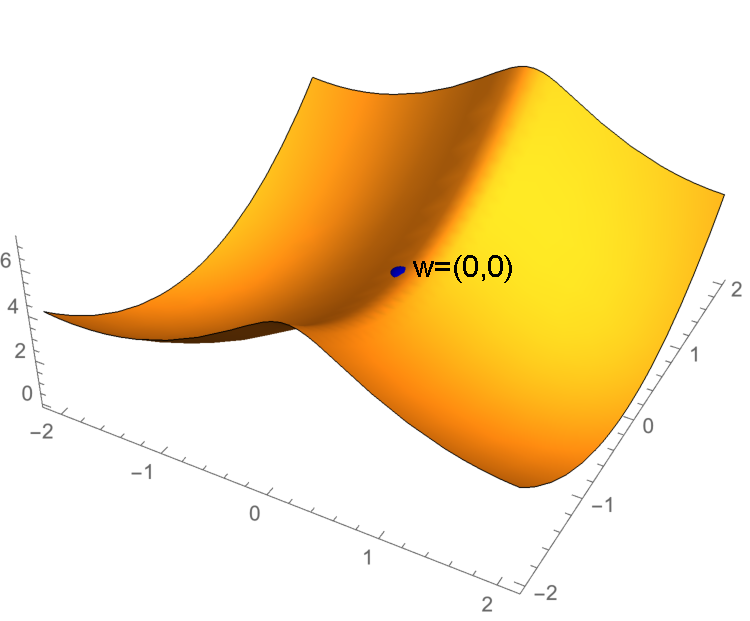
\includegraphics[width=0.8\linewidth]{Untitled-1.pdf}
\end{minipage}
\begin{minipage}[t]{0.5\linewidth}
\centering
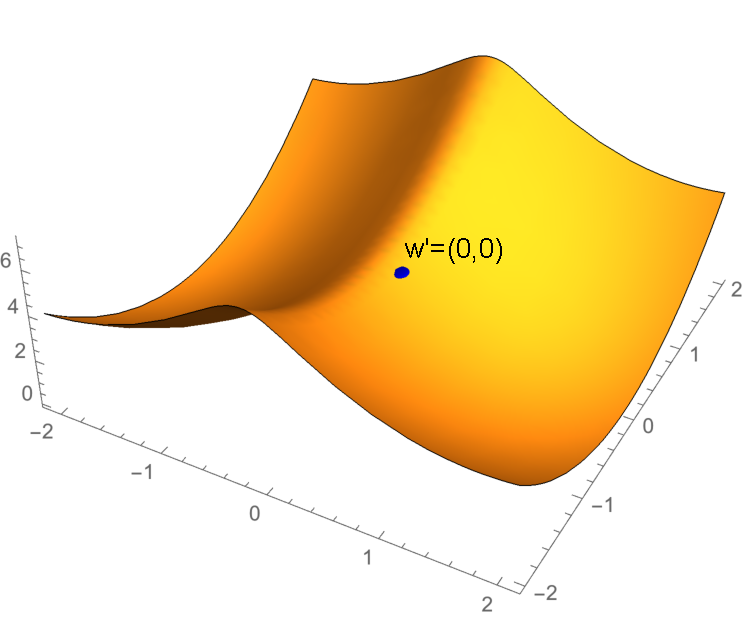
\includegraphics[width=0.8\linewidth]{Untitled-2.pdf}
\end{minipage}
\caption{Illustration of "Fence-Sitting" Situation for Stability of Non-convex Optimization}\label{illustration}
\end{figure}

To guarantee stability, we need $\bm{w}_k$ to randomly decide which side to go when it comes close to the ridge. The noise needs to be isotropic and smooth enough in order to cross this ridge, as the direction of variation can be quite arbitrary. SGLD successfully tackles the fence-sitting problem by smoothing the probability of going either side, and adding noise to subsequent steps to avoid unstable shallow local minima. The bounds for SGD in~\citet{hardt2015train} also exploits randomness of choosing $i_k$, but the noise is not smooth enough. So their bound requires the subsequent steps to be very small, to keep $w_k$ not far from the ridge.\\

\section{Backgrounds on Fokker-Planck Equation}\label{Background-fokker-planck}

It is known that that the movement of a particle in the $d$-dimensional space influenced by its current state and random forces (here we only consider a simple case), can be characterized by the following stochastic differential equation (SDE):
\begin{equation}
 d\X_t = \bm{\mu}(\X_t, t)dt + \sqrt{2 \beta^{-1}} d\B_t
\end{equation}
where $\X_t$ is the random position of the particle at time $t$, $\bm{\mu}(\X_t, t)$ is the $d$-dimensional random drift vector, and $B_t$ is the $d$ dimensional Brownian motion. Denote the density function of $\X_t$ as $p(\x,t)$, then Fokker-Planck equation describes the evolution of $p(\x,t)$:
\begin{equation}
 \frac{\partial p(\x,t)}{\partial t} = \frac{1}{\beta}\Delta p(\x, t) - \bm{\nabla}\cdot(p(\x,t)\bm{\mu}(\x, t))
 %-\sum_{i=1}^d \frac{\partial}{\partial x_i}[\mu_i(\x_t, t)p(\x, t)] + \frac{1}{2} \sum_{i,j=1}^d \frac{\partial^2}{\partial x_i \partial x_j}[p(\x,t)]
\end{equation}
where $\Delta$ is the Laplace operator.

For Gaussian distribution, we have the following log-Sobolev inequality, which relates Fisher information and KL divergence.
\begin{theorem}
	For $\gamma=\mathcal{N}(0,\sigma_0^2I)$ and any distribution $\pi$ which has absolute continuous density, we have:
	\begin{equation}
		\mathbb{E}_{\pi}\left(\log \frac{\pi}{\gamma}\right)\leq \sigma_0^2 \mathbb{E}_{\pi}\left\Vert\bm{\nabla} \log \frac{\pi}{\gamma}\right\Vert^2
	\end{equation}
\end{theorem}

A special case of Langevin equation is Ornstein-Uhlenbeck process, which plays a critical role in our discretization construction.
\begin{proposition}\label{ornstein-uhlenbeck}
	An Ornstein-Uhlenbeck process is solution to the following SDE:
	\begin{equation}
		d\bm{X}_t=\lambda(\bm{b}-\bm{X}_t)dt+\sqrt{\frac{2}{\beta}}d\bm{B}_t,
	\end{equation}
	for some constant vector $\bm{b}\in \mathbb{R}^d$ and constant $\lambda>0$.
	Its Fokker-Planck equation is:
	\begin{equation}
\frac{\partial\pi}{\partial t}=\frac{1}{\beta}\Delta \pi+\lambda\bm{\nabla}\cdot\left((\bm{w}-\bm{b})\pi\right),
\end{equation}
and the solution can be directly written as:
\begin{equation}
	\bm{X}_t=e^{-\lambda t}\bm{X}_0+\left(1-e^{-\lambda t}\right)\bm{b}+\sqrt{\frac{2}{\beta}}\int_{0}^t e^{-\lambda(t-s)}d\bm{B}_s
\end{equation}
\end{proposition}
The proof can be found in any standard textbook about Fokker-Planck equations, see, e.g.~\citep{risken1996fokker}
\section{Omitted Proofs in Section 2}

\textbf{Proof of theorem \ref{PAC-Bayesian}}
\begin{proof}
	For simplicity, we replace $\ell(\w,z)$ with $\ell(\w,z)-\mathbb{E}_{\mathcal{D}\times \mathcal{P}}\ell(\w,z)$, and assume the distribution of loss function is centered under data distribution and the prior. It is easy to check that this modification does not affect following analysis.

	We use the Donsker-Varadhan change of measure inequality: for any pair of distributions $\mathcal{P}$ and $\mathcal{Q}$ and functional $\phi$, we have
\begin{equation}\label{donsker-varadhan}
	\mathbb{E}_{\mathcal{Q}} (\phi(\ell))\leq D_{KL}(\mathcal{Q}||\mathcal{P})+\ln\mathbb{E}_{\mathcal{P}} \left(e^{\phi(\ell)}\right)
\end{equation}
Consider functions $\phi(\ell)$ in the form of $\phi(w)=\lambda\left(\mathbb{E}\ell(w;z)-\hat{\mathbb{E}}_n \ell(w;z)\right)$ (function class of $\ell(w,\cdot)$ indexed by $w$), while the values of $\lambda$ will be determined later. (The notation $\hat{\mathbb{E}}_n$ denotes empirical expectation, i.e., $\hat{\mathbb{E}}_n h(x)=\frac{1}{n}\sum_{i=1}^n h(x_i)$)

For any fixed $\lambda>0,\delta'>0$, by Markov inequality we have the following with probability $1-\delta'$
\begin{equation}
	\mathbb{E}_{\mathcal{P}}\left(e^{\lambda\left(\mathbb{E}\ell(w;z)-\hat{\mathbb{E}}_n \ell(w;z)\right)}\right)\leq \frac{1}{\delta'}\mathbb{E}_{S}\mathbb{E}_{\mathcal{P}}\left(e^{\lambda\left(\mathbb{E}\ell(w;z)-\hat{\mathbb{E}}_n \ell(w;z)\right)}\right)
\end{equation}
For any finite set $\Lambda\subseteq \mathbb{R}^+,\delta>0$, let $\delta'=\frac{\delta}{|\Lambda|}$, we have:
\begin{equation}\label{union-bound-ineq}
	\forall \lambda\in\Lambda,\quad\mathbb{P}\left(\mathbb{E}_{\mathcal{P}}\left(e^{\lambda\left(\mathbb{E}\ell(w;z)-\hat{\mathbb{E}}_n \ell(w;z)\right)}\right)> \frac{|\Lambda|}{\delta}\mathbb{E}_{S}\mathbb{E}_{\mathcal{P}}\left(e^{\lambda\left(\mathbb{E}\ell(w;z)-\hat{\mathbb{E}}_n \ell(w;z)\right)}\right)\right)\leq \frac{\delta}{|\Lambda|}
\end{equation}
 and by union bound,
\begin{equation}
	\quad\mathbb{P}\left(\exists \lambda\in \Lambda,\mathbb{E}_{\mathcal{P}}\left(e^{\lambda\left(\mathbb{E}\ell(w;z)-\hat{\mathbb{E}}_n \ell(w;z)\right)}\right)> \frac{|\Lambda|}{\delta}\mathbb{E}_{S}\mathbb{E}_{\mathcal{P}}\left(e^{\lambda\left(\mathbb{E}\ell(w;z)-\hat{\mathbb{E}}_n \ell(w;z)\right)}\right)\right)\leq |\Lambda|\delta'=\delta
\end{equation}
Let $S'=\{x_1',x_2',\cdots,x_n'\}$ be an independent copy of $n$ samples, and let $\hat{\mathbb{E}}_n'$ denotes empirical expectation with respect to $S'$, i.e., $\hat{\mathbb{E}}_n' h(x)=\frac{1}{n}\sum_{i=1}^n h(x_i')$. We have
\begin{equation}
\mathbb{E}_{S}\left(e^{\lambda\left(\mathbb{E}\ell(w;z)-\hat{\mathbb{E}}_n \ell(w;z)\right)}\right)=\mathbb{E}_{S}\left(e^{\mathbb{E}_{S'}\lambda\left(\hat{\mathbb{E}}'_n \ell(w;z)-\hat{\mathbb{E}}_n\ell(w;z)\right)}\right)\leq \mathbb{E}_{S,S'}\left(e^{\lambda\left(\hat{\mathbb{E}}'_n \ell(w;z)-\hat{\mathbb{E}}_n\ell(w;z)\right)}\right)
\end{equation}
The last inequality is due to convexity of exponential function and Jensen's Inequality.

Given $\lambda$ fixed, we can expand the right hand side based on independence, and each term is upper bounded by $\exp\left(\frac{\lambda^2s^2}{n^2}\right)$ by subGaussian assumption. Putting them together, we have:
\begin{equation}
\mathbb{E}_{S,S',\mathcal{P}}\left(e^{\lambda\left(\hat{\mathbb{E}}'_n \ell(w;z)-\hat{\mathbb{E}}_n\ell(w;z)\right)}\right)=\prod_{i=1}^n \mathbb{E}\left(e^{\frac{\lambda}{n}\left( \ell(w;z_i')-\ell(w;z_i)\right)}\right)\leq e^{\frac{\lambda^2s^2}{n}}
\end{equation}
Combining two inequalities above, we have the following bound:
\begin{equation}
	\mathbb{E}_{S,\mathcal{P}}\left(e^{\lambda\left(\mathbb{E}\ell(w;z)-\hat{\mathbb{E}}_n \ell(w;z)\right)}\right)\leq e^{\frac{\lambda^2s^2}{n}}
\end{equation}
Using Equation~(\ref{union-bound-ineq}), we have the following with probability $1-\delta$:
\begin{equation}
	\forall \lambda\in\Lambda,\quad\mathbb{E}_{\mathcal{P}}\left(e^{\lambda\left(\mathbb{E}\ell(w;z)-\hat{\mathbb{E}}_n \ell(w;z)\right)}\right)\leq \frac{|\Lambda|}{\delta}e^{\frac{\lambda^2s^2}{n}}
\end{equation}
Combined with Equation~(\ref{donsker-varadhan}) by letting $\phi_{\lambda}(w)=\lambda\left(\mathbb{E}\ell(w;z)-\hat{\mathbb{E}}_n \ell(w;z)\right)$ for different values of $\lambda\in\Lambda$, for any posterior $\mathcal{Q}$, we have the following result with probability $1-\delta$:
\begin{equation}\label{lambda-ineq}
	\forall\lambda\in\Lambda,\quad \mathbb{E}_{\mathcal{Q}}\left(\mathbb{E} \ell(w;z)- \hat{\mathbb{E}}_n \ell(w;z)\right)\leq \frac{1}{\lambda}\left(D_{KL}(\mathcal{Q}||\mathcal{P})+\log \frac{|\Lambda|}{\delta}\right)+\frac{\lambda s^2}{n}
\end{equation}

Take $\Lambda=\left\{\frac{1}{s}\sqrt{n\left(2^i+\log\frac{1}{\delta}+\log \log M\right)}\right\}_{i=1}^{\lceil\log M\rceil}$ with $|\Lambda|=\lceil\log M\rceil$. For any posterior $\mathcal{Q}\in \Xi$, $D_{KL}(\mathcal{Q}||\mathcal{P})\leq M$. Choose the index $i\in\{1,2,\cdots, \lceil\log M\rceil\}$ such that $2^i\leq D_{KL}(\mathcal{Q}||\mathcal{P})<2^{i+1}$ (if $D_{KL}(\mathcal{Q}||\mathcal{P})<2$, let $i=1$) and plug the corresponding value of $\lambda$ into Equation~(\ref{lambda-ineq}), we can easily get the following upper bound for the right hand side:
\begin{equation}
	 \frac{1}{\lambda}\left(D_{KL}(\mathcal{Q}||\mathcal{P})+\log \frac{|\Lambda|}{\delta}\right)+\frac{\lambda s^2}{n}\leq 2s\sqrt{\frac{D_{KL}(\mathcal{Q}||\mathcal{P})\vee 1+\log \frac{1}{\delta}+\log\log M}{n}},\quad \forall \mathcal{Q}\in \Xi
\end{equation}
So the theorem is proven.
\end{proof}
Remark: if we choose a single value of $\lambda$ fixed, the proof becomes the same as~\cite{germain2016pac}, which is based on Donsker-Varadhan change-of-measure inequality. But their bound does not give optimal dependence on KL divergence. In order to overcome this difficulty, we use a set of values for $\lambda$ and union bound to obtain the $\sqrt{\frac{D_{KL}}{n}}$ bound, at a price of double logarithmic term.

\section{Omitted Proofs in Section 3}

\textbf{Proof of Lemma \ref{stability bound by Hellinger} }
\begin{proof}
\begin{equation}\label{stability-to-hellinger}
\begin{split}
\epsilon_n=&\sup_{z,S,S'}\left|\int_{\mathbb{R}^d}\ell(\bm{w};z)\pi(\bm{w})dw-\int_{\mathbb{R}^d}\ell(\bm{w};z)\pi'(\bm{w})dw\right|\\
  =&\sup_{z,S,S'}\left|\int_{\mathbb{R}^d}\ell(\bm{w};z)\left(\sqrt{\pi}+\sqrt{\pi'}\right)\left(\sqrt{\pi}-\sqrt{\pi'}\right)dw\right|\\
  \leq&\sup\left\{\left(\int_{\mathbb{R}^d}\ell(\bm{w};z)^2\left(\sqrt{\pi}+\sqrt{\pi'}\right)^2dw\right)^{\frac{1}{2}}\left(\int_{\mathbb{R}^d}\left(\sqrt{\pi}-\sqrt{\pi'}\right)^2dw\right)^{\frac{1}{2}}\right\}\\
  =&2\sup_{\pi} \Vert \ell\Vert_{L^2(\pi)}\sqrt{D_{H}(\pi||\pi')}\\
  \leq& 2C\sqrt{D_{H}(\pi||\pi')}\\
  \end{split}
\end{equation}
\end{proof}

\noindent \textbf{Proof of Proposition \ref{stability-bound-continuous}}
\begin{proof}
According to the analysis above, we only need to bound $D_H(\pi||\pi')$ from above.

Apparently, at time $t=0$, $D_H(\pi||\pi')=0$. We then estimate $\frac{d}{dt}D_{H}(\pi_t||\pi_t')$:
\begin{equation}
\begin{split}
\frac{d}{dt}D_{H}(\pi_t||\pi_t')=&-\int_{\mathbb{R}^d} \frac{\partial }{\partial t}\sqrt{\pi \pi'}dw\\
&=-\int_{\mathbb{R}^d}\frac{\sqrt{\pi'}}{2\sqrt{\pi}}\frac{\partial \pi}{\partial t}dw-\int_{\mathbb{R}^d}\frac{\sqrt{\pi}}{2\sqrt{\pi'}}\frac{\partial \pi'}{\partial t}dw\\
&=-\int_{\mathbb{R}^d}\frac{\sqrt{\pi'}}{2\sqrt{\pi}}\left(\frac{1}{\beta}\Delta \pi+\bm{\nabla}\cdot(\pi \bm{\nabla}F_n)\right)dw-\int_{\mathbb{R}^d}\frac{\sqrt{\pi}}{2\sqrt{\pi'}}\left(\frac{1}{\beta}\Delta \pi'+\bm{\nabla}\cdot(\pi' \bm{\nabla}F_n')\right)dw\\
&=\frac{1}{2}\int_{\mathbb{R}^d}\bm{\nabla}\frac{\sqrt{\pi'}}{\sqrt{\pi}}\cdot\left(\frac{1}{\beta}\nabla\pi+\pi \bm{\nabla}F_n\right)dw+\frac{1}{2}\int_{\mathbb{R}^d}\bm{\nabla}\frac{\sqrt{\pi}}{\sqrt{\pi'}}\left(\frac{1}{\beta}\bm{\nabla}\pi'+\pi' \bm{\nabla}F_n')\right)dw\\
\end{split}
\end{equation}
The last equality is due to integration by parts. Technical conditions such as uniform decaying tails of $\pi$ and $\pi'$ can be found in~\citep{risken1996fokker}. We then proceed to calculate the part induced by gradient update (with coefficient $1$) and those induced by Gaussian convolution (with coefficient $\frac{1}{\beta}$) individually, which can be described as follows:
\begin{equation}
\begin{split}
\frac{d}{dt}D_{H}(\pi_t||\pi_t')&=\frac{1}{2}\int_{\mathbb{R}^d}\bm{\nabla}\frac{\sqrt{\pi'}}{\sqrt{\pi}}\cdot\left(\frac{1}{\beta}\nabla\pi+\pi \bm{\nabla}F_n\right)dw+\frac{1}{2}\int_{\mathbb{R}^d}\bm{\nabla}\frac{\sqrt{\pi}}{\sqrt{\pi'}}\left(\frac{1}{\beta}\bm{\nabla}\pi'+\pi' \bm{\nabla}F_n')\right)dw\\
&=\frac{1}{4}\int_{\mathbb{R}^d}\sqrt{\pi \pi'}\bm{\nabla}\log\frac{\pi'}{\pi}\cdot\left(\frac{1}{\beta}\bm{\nabla}\log\pi+ \bm{\nabla}F_n\right)dw+\frac{1}{4}\int_{\mathbb{R}^d}\sqrt{\pi \pi'}\bm{\nabla}\log\frac{\pi}{\pi'}\cdot\left(\frac{1}{\beta}\bm{\nabla}\log\pi'+\bm{\nabla}F_n')\right)dw\\
&=-\frac{1}{4}\int_{\mathbb{R}^d}\sqrt{\pi \pi'}\left(\frac{1}{\beta}\|\bm{\nabla}\log\frac{\pi'}{\pi}\|^2+\bm{\nabla}\log\frac{\pi}{\pi'}\cdot(\bm{\nabla}F_n-\bm{\nabla}F_n')\right)dw\\
&\le\frac{1}{4}\int_{\mathbb{R}^d}\frac{\beta}{4}\sqrt{\pi \pi'}\|\bm{\nabla}F_n-\bm{\nabla}F_n'\|^2dw\\
&\le \frac{\beta L^2}{16n^2}
\end{split}
\end{equation}
Integrating through time and plugging into the estimate above, we have:
\begin{equation}
  \epsilon_n\leq 2C \sqrt{D_H(\pi_T||\pi'_T)}\leq \frac{LC\sqrt{\beta T}}{2n}
\end{equation}
\end{proof}

\noindent \textbf{Proof of Proposition \ref{ideal-pac-bayes-2}}
\begin{proof}
We only need to bound the KL divergence to prior distribution $\gamma$.
\begin{equation}
\begin{split}
\frac{d}{dt}D_{KL}(\pi_t||\gamma)=&\int_{\mathbb{R}^d} \frac{\partial \pi}{\partial t}(\log \pi+1-\log \gamma)dw\\
=&-\frac{1}{\beta}\int_{\mathbb{R}^d} \pi\Vert \bm{\nabla} \log \pi-\bm{\nabla}\log\gamma\Vert^2dw - \int_{\mathbb{R}^d} \pi\langle \bm{\nabla}\hat{\mathbb{E}}_n f(\bm{w})+\lambda \bm{w}+\frac{1}{\beta}\bm{\nabla} \log \gamma, \bm{\nabla} \log \pi-\bm{\nabla} \log \gamma\rangle dw\\
\leq &-\left(\frac{1}{\beta}-\frac{1}{2C}\right)\int_{\mathbb{R}^d} \pi\Vert \bm{\nabla} \log \pi-\bm{\nabla}\log\gamma\Vert^2dw+\frac{C}{2}\int_{\mathbb{R}^d} \pi \Vert \bm{\nabla}\hat{\mathbb{E}}_n f(\bm{w})+\lambda\bm{w}+\frac{1}{\beta}\bm{\nabla}\log \gamma\Vert^2dw
\end{split}
\end{equation}
We use Cauchy-Schwartz inequality in the second step, and the constant $C$ will be determined later.
The first term is minus Fisher information $I(\pi||\gamma)$, which can be upper bounded by $-D_{KL}(\pi||\gamma)$ itself using logarithmic Sobolev inequality~\citep{gross1975logarithmic,markowich2000trend}:
\begin{equation}
D_{KL}(\pi||\gamma)\leq \sigma_0^2I(\pi||\gamma),\quad\text{for } \gamma=\mathcal{N}(0,\sigma_0^2I)
\end{equation}
Let $C=\beta$ and plug into the log Sobolev inequality, we get:
\begin{equation}
  \frac{d}{dt}D_{KL}(\pi_t||\gamma)\leq -\frac{1}{2\beta\sigma_0^2}D_{KL}(\pi_t||\gamma)+\frac{\beta}{2}\int_{\mathbb{R}^d} \pi_t \Vert \bm{\nabla}\hat{\mathbb{E}}_n f(\bm{w})+\lambda \bm{w}+\frac{1}{\beta}\bm{\nabla}\log \gamma\Vert^2dw
\end{equation}
Solving for $D_{KL}$ with initial value $D_{KL}(\pi_0||\gamma)=0$, we get:
\begin{equation}
  D_{KL}(\pi_T||\gamma)\leq \frac{\beta}{2}\int_{0}^T e^{\frac{-(T-t)}{2\beta \sigma_0^2}}\mathbb{E}_{\pi_t} \left\Vert \bm{\nabla}\hat{\mathbb{E}}_n f(\bm{w})+\lambda\bm{w}+\frac{1}{\beta}\bm{\nabla}\log \gamma\right\Vert^2dt
\end{equation}
Since we use Gaussian prior, the second term in the expectation can be directly calculated as $\frac{1}{\beta}\bm{\nabla}\log \gamma=-\frac{1}{\beta\sigma_0^2}\bm{w}$, which exactly cancel out with the $\lambda\bm{w}$ term. So we have:
\begin{equation}
  D_{KL}(\pi_T||\gamma)\leq \frac{\beta}{2}\int_{0}^T e^{\frac{-\lambda(T-t)}{2}}\mathbb{E}_{\pi_t} \Vert \bm{\nabla}\hat{\mathbb{E}}_n f(\bm{w})\Vert^2dt
\end{equation}
\end{proof}
Remark: if we do not add the $\ell_2$ regularization term, the bound will become
\begin{equation}
  D_{KL}(\pi_T||\gamma)\leq \frac{\beta}{2}\int_{0}^T e^{\frac{-(T-t)}{2\beta \sigma_0^2}}\mathbb{E}_{\pi_t} \left\Vert \bm{\nabla}F_n+\frac{1}{\beta}\bm{\nabla}\log \gamma\right\Vert^2dt,
\end{equation}
which directly depends on norm of the parameter. This is undesirable in high dimensions, since the diffusion term will make the norm at least $\Omega(d)$. Therefore, the use of $\ell_2$ regularization is critical to our analysis.
\section{Omitted Proofs in Section 4}
\subsection{Stability of Langevin Monte Carlo}\label{section: langevinMC}
We consider the following LMC algorithm, which uses full gradients in each update.

\begin{equation}
  \bm{w}_{k+1}=\bm{w}_k-\frac{\eta_k}{n}\sum_{i=1}^n\bm{\nabla} f(\bm{w}_k;z_i)+\sqrt{\frac{2\eta_k}{\beta}} \mathcal{N}(0,I_d)
\end{equation}

Suppose two neighboring datasets $S,S'$ differing only in the $i_*$-th data. Then one can divide each iteration into two parts: the first part just update $\w_k$ and $\w_k'$ with gradients over $n-1$ same data and $z_{i_*}$, i.e. 
\begin{equation}
  \w_k^{(1)} := \w_k - \frac{\eta_k}{n}\sum_{i \neq i_*} \bm{\nabla} f(\bm{w}_k;z_i)- \frac{\eta_k}{n}\bm{\nabla} f(\bm{w}_k;z_{i_*}) 
\end{equation},
\begin{equation}
  \w_k^{(1)\prime} := \w_k' - \frac{\eta_k}{n}\sum_{i \neq i_*} \bm{\nabla} f(\bm{w}_k';z_i)- \frac{\eta_k}{n}\bm{\nabla} f(\bm{w}_k';z_{i_*}) 
 \end{equation} and then we obtain $\bm{w}_{k+1}$ and $\bm{w}_{k+1}'$ by adding Gaussian noise and replacing the gradient of sample $z_{i_*}$ in $\bm{w}_k^{(1)\prime}$ by the gradient of sample $z_{i_*}'$, i.e. $\w_{k+1}' = {\w_k^{(1)\prime}} - \frac{\eta_k}{n} \bm{\nabla} (f(\bm{w}_k;z_{i_*}')-f(\bm{w}_k;z_{i_*})) + \sqrt{\frac{2\eta_k}{\beta}} \mathcal{N}(0,I_d)$.
In the first step, squared Hellinger distance does not increase because of the non-expansive property. For the second step, one can view them as consecutive SDEs with drift term $\bm{g},\bm{g}'$ of order $O(\frac{1}{n})$. Hence we can prove the increments of $D_H(\pi||\pi')$ after one iteration is of order $O(\frac{1}{n^2})$, which leads to the following generalization bound.

\begin{theorem}[Generalization Error of LMC]
\label{generalization LMC}
  Assuming that
  $$\forall z,z',\forall\bm{w},\|\bm{\nabla}f(\bm{w};z)-\bm{\nabla}f(\bm{w};z')\|\le L$$

  Let $\bm{w}_N$ be result of LMC at $N$-th round. If loss function $\ell(\cdot,\cdot)$ is uniformly bounded by constant, then the following inequality holds:
  \begin{equation}
    \mathbb{E}[\mathrm{err}_{gen}(\bm{w}_T)]\leq O\left(\frac{L\sqrt{\beta\sum_{k=1}^N \eta_k}}{n}\right)
  \end{equation}
  where the expectation is taken over the randomness of training data.
\end{theorem}

\begin{proof}
  Here we bound uniform stability of full gradient SGLD by estimating squared Hellinger distance.

We shall assume $\|\bm{\nabla} f_i\|\le L$ (which can actually be relaxed to $\|\bm{\nabla} (f_i-f_j)\|\le 2L$). (In the proof we will use $f_i(\w)$ for abbreviation of $f(\w,z_i)$, and $f_i'(w)$ for $f(\w,z_i')$. The prime notation on $f$ does not stand for derivative, which is always denoted using $\bm{\nabla}$ operator.)

Suppose at step $k$, the starting parameters are $W_{k-1}$ and $W'_{k-1}$ resp. The ending parameters are given by
\begin{equation}
  \bm{w}_{k+1}=\bm{w}_{k}-\frac{\eta_k}{n}\sum\limits_{i=1}^n\bm{\nabla} f_i(\bm{w}_{k})+\sqrt{\frac{2\eta_k}{\beta}}\bm{B}_k
\end{equation}
\begin{equation}
  \bm{w}_{k+1}'=\bm{w}_{k}'- \frac{\eta_k}{n}\left(\bm{\nabla} f_{i_*}'(\bm{w}'_{k})+\sum\limits_{i=1,i\neq i_*}^n\bm{\nabla} f_i(\bm{w}_{k}')\right)+\sqrt{\frac{2\eta_k}{\beta}}\bm{B}_k'
\end{equation}

where $\bm{B}_k, \bm{B}_k'\sim \mathcal{N}(0, I_d)$.

We consider a family of random variable $\bm{\theta}_t,\bm{\theta}_t'(0\le t\le \eta_k)$ defined by
\begin{equation}
  \bm{\theta}_t=\bm{w}_{k}- \frac{\eta_k}{n}\sum\limits_{i=1}^n\bm{\nabla} f_i(\bm{w}_{k})+\sqrt{\frac{2t}{\beta}}\bm{B}_k
\end{equation}
\begin{equation}
  \bm{\theta}_t'=\bm{w}_{k}'- \frac{\eta_k}{n}\sum\limits_{i=1}^n\bm{\nabla} f_i(\bm{w}_{k}')- \frac{t}{n}\Big(\bm{\nabla} f_{i_*}'(\bm{w}_k')-\bm{\nabla}f_{i_*}(\bm{w}_k')\Big)+\sqrt{\frac{2t}{\beta}}\bm{B}_k'
\end{equation}
Till now, we only consider the one-time distribution of $\bm{\theta}_t,\bm{\theta}_t'$, and their dependence on $\bm{w}_k,\bm{w}_k'$, without taking the inter-dependence of whole process into consideration, so we use a simple way of expanding the Gaussian noise. In the actual construction of the SDE, it will be expanded via Brownian motion.

Let the pdf of $\bm{\theta}_t, \bm{\theta}_t'$ be $\pi_t, \pi_t'$. We can see that
\begin{itemize}
  \item $\bm{\theta}_0=\bm{w}_{k}- \frac{\eta_k}{n}\sum\limits_{i=1}^n\bm{\nabla} f_i(\bm{w}_{k}),\bm{\theta}_0'=\bm{w}_{k}'- \frac{\eta_k}{n}\sum\limits_{i=1}^n\bm{\nabla} f_i(\bm{w}_{k}')$, so that
  \begin{equation}
    D_H(\pi_0||\pi_0')\le D_H(p_k||p_k')
  \end{equation}
\item the explicit formulae for $\pi_t$ and $\pi_t'$ are given by
\begin{equation}
  \pi_t(\bm{w})=\mathbb{E}_{\bm{w}_k}\left(\frac{\beta}{4 \pi t}\right)^{d/2} \exp\Big(-\frac{\beta}{4t}\Vert\bm{w}-\bm{w}_k+\frac{\eta}{n}\sum\limits_{i=1}^n\bm{\nabla} f_i(\bm{w}_{k})\Vert^2\Big)
\end{equation}
and
\begin{equation}
  \pi_t'(\bm{w})=\mathbb{E}_{\bm{w}_k'}\left(\frac{\beta}{4 \pi t}\right)^{d/2} \exp\Big(-\frac{\beta}{4t}\Vert\bm{w}-\bm{w}_k'+\frac{\eta}{n}\sum\limits_{i=1}^n\bm{\nabla} f_i(\bm{w}_{k}')+ \frac{t}{n}\left(\bm{\nabla} f_{i_*}'(\bm{w}_k')-\bm{\nabla}f_{i_*}(\bm{w}_k')\right)\Vert^2\Big)
\end{equation}


Although formidable at first glance, $\pi_t$ and $\pi_t'$ are nothing but superposition of Gaussian density functions w.r.t $\bm{w}$.


Define $\bm{g}_t(\bm{w})$ to be $\bm{0}$ and define $\bm{g}_t'(\bm{w})$ by 
\begin{equation}
\begin{split}
  &\mathbb{E}_{\bm{w}_k'}[\frac{1}{n}\left(\bm{\nabla} f_{i_*}'(\bm{w}_k')-\bm{\nabla}f_{i_*}(\bm{w}_k')\right)|\bm{\theta}_t'=\bm{w}]\\
  =& \frac{1}{n\pi_t'(\bm{w})}\mathbb{E}_{\bm{w}_k'}\left(\left(\bm{\nabla} f_{i_*}'(\bm{w}_k')-\bm{\nabla}f_{i_*}(\bm{w}_k')\right)\left(\frac{\beta}{4 \pi t}\right)^{d/2} e^{-\frac{\beta}{4t}\Vert\bm{w}-\bm{w}_k'+\frac{\eta}{n}\sum\limits_{i=1}^n\bm{\nabla} f_i(\bm{w}_{k}')+ \frac{t}{n}\left(\bm{\nabla} f_{i_*}'(\bm{w}_k')-\bm{\nabla}f_{i_*}(\bm{w}_k')\right)\Vert^2}\right)
\end{split}
\end{equation}

Then by taking derivatives w.r.t to $\bm{w}$ and $t$, we can obtain the following equations, which has the same one-time marginal distribution as $\bm{\theta}_t$ and $\bm{\theta}_t'$ (though they are not the same process):
\begin{equation}
  \frac{\partial \pi_t}{\partial t}=\frac{1}{ \beta}\Delta \pi_t+\bm{\nabla}\cdot\left(\pi_t \bm{g}_t\right)
\end{equation}
\begin{equation}
  \frac{\partial \pi_t'}{\partial t}=\frac{1}{ \beta}\Delta \pi_t'+\bm{\nabla}\cdot\left(\pi_t'\bm{g}_t'\right)
\end{equation}
\end{itemize}

From definition and the assumption $\forall z,z', \|\nabla f(\bm{w};z)-\nabla f(\bm{w};z')\|\le L$, we have
\begin{equation}
  \forall \bm{w},\|\bm{g}_t(\bm{w})-\bm{g}_t'(\bm{w})\|\le \frac{L}{n}
\end{equation}

\begin{align*}
\frac{d}{dt}D_{H}(\pi_t||\pi'_t)&=-\frac{1}{2}\int_{\mathbb{R}^d} \left(\frac{1}{ \beta}\sqrt{\pi \pi'}\|\bm{\nabla}\log \frac{\pi}{\pi'}\|^2 + \sqrt{\pi \pi'}\bm{\nabla}\log \frac{\pi}{\pi'}\cdot(\bm{g}_t-\bm{g}_t')\right)dw\\
&\le \frac{\beta}{8} \int_{\mathbb{R}^d} \sqrt{\pi \pi'}\|\bm{g}_t-\bm{g}_t'\|^2dw\\
&=\frac{\beta L^2}{8n^2}
\end{align*}

As a result, we can estimate the change of squared Hellinger distance in this step:
\begin{align*}
D_H(\pi_{k+1}||\pi_{k+1}')&=D_H(\pi_{\eta_k}||\pi_{\eta_k}')\\
&=D_H(\pi_{0}||\pi_{0}')+\int_0^{\eta_k} \frac{d}{dt}D_{H}(\pi_t||\pi'_t)dt\\
&\le D_H(p_{0}||p_0')+\int_0^{\eta_k} \frac{\beta L^2}{8n^2}dt\\
&= D_H(p_{0}||p_0')+ \frac{\beta L^2}{8n^2}\eta_k\\
\end{align*}

Then by induction we shall have a final bound for $D_{KL}(\pi||\pi')$ of the form $\frac{\beta L^2}{8n^2}\sum\limits_{k=1}^N \eta_k $.

Then the bound for uniform stability is given by
\begin{equation}
  \epsilon_n\leq O\left(\frac{L\sqrt{\beta\sum_{k=1}^N \eta_k}}{n}\right)
\end{equation}
\end{proof}
Combining the techniques from the proof of Theorem~\ref{generalization LMC} and Lemma~\ref{Hellinger - improved}, we can easily get the general result for the case of mini-batch.

\subsection{Stability of SGLD - A Succinct Analysis}\label{section-succinct}
As random draw of a training example is more popular in practice, it is desirable to analyze generalization properties of SGLD. In the rest part of this section, we will assume $\bm{g}_k=\bm{\nabla} f_{i_k}(\bm{w})$, where $i_k$ is the index of randomly drawn training example. We will first present a simple analysis for stability of SGLD. Though the resulting bound is not optimal, the analysis illustrates important principles for understanding how SGLD helps stability. In the following, we will derive upper bounds for $\delta_k\triangleq D_H(p_k||p_k')$ recursively. There are two possible cases for $i_k$:
\begin{itemize}
  \item If $i_k\neq i_*$, then SGLD implemented over $S$ or $S'$ will use the same gradient mapping, i.e. $\psi_k: \bm{w}\mapsto \bm{w}-\eta_k\nabla f(\bm{w};z_{i_k})$, then we have 
  \begin{equation}
  D_{H}(\mathcal{P}(\psi_k (\bm{w}_k)|i_k)||\mathcal{P}(\psi_k (\bm{w}_k')|i_k))\leq D_{H}(p_k||p_k')=\delta_k
  \end{equation}
  Furthermore let $\mathcal{G}_k=\mathcal{N}(0,\frac{\eta_k}{\beta}I_d)$, by the convexity of squared Hellinger distance (which is implied by joint convexity of $f$-divergence), there is 
  \begin{align*}
  D_H(\mathcal{P}(\bm{w}_{k+1}|i_k)||\mathcal{P}(\bm{w}'_{k+1}|i_k))&=D_H(\mathcal{G}_k*\mathcal{P}(\psi_k (\bm{w}_k)|i_k)||\mathcal{G}_k*\mathcal{P}(\psi_k (\bm{w}_k')|i_k))\\
  &\le D_{H}(\mathcal{P}(\psi_k (\bm{w}_k)|i_k)||\mathcal{P}(\psi_k (\bm{w}_k')|i_k))\\
  &\le \delta_k
  \end{align*}
  So in this case, the SGLD update is non-expansive with respect to $\delta_k$.

  \item If $i_k=i_*$, we have nothing but limited step size in hand. The increase of $f$-divergence can be bounded through norm-based shifts in parameter space only under smoothness conditions, which is helped by Gaussian noise. Therefore, we expand the discrete-time update into a stochastic process, where the effect of gradient flow is smoothed by Gaussian at each time $t$.
\end{itemize}

Concretely, for $i_k=i_*$, the update can be interpolated as:
\begin{equation}
\forall t\in[0,\eta_k],\quad\bm{\theta}_t=\bm{\theta}_0-\int_0^t \bm{\nabla} f_{i_k}(\bm{\theta}_0)ds+\sqrt{\frac{2}{\beta}}\int_0^td\bm{B}_s,\quad \bm{\theta}_0=\bm{w}_k
\end{equation}
However, $\bm{\theta}_t$ is not a Markov process, as it always involves the initial random point $\bm{\theta}_0$. Using the same technique as in \cite{raginsky2017non}, we define $\bm{g}_t(\bm{v})\triangleq\mathbb{E}\left(\bm{\nabla} f_{i_k}(\bm{\theta}_0)\Big| \bm{\theta}_t=\bm{v}\right)$. Mimicking distribution results~\citep{gyongy1986mimicking} guarantees solution to the following SDE has the same one-time marginal as $\bm{\theta}_t$.
\begin{equation}
\begin{split}
  d\bm{v}_t = \bm{g}_s(\bm{v}_s)ds+\sqrt{\frac{2}{\beta}}d\bm{B}_s,\quad v_0\sim p_k
  \end{split}
\end{equation}
The corresponding Fokker-Planck equation for above process is:
\begin{equation}
  \frac{\partial \pi}{\partial t}=\bm{\nabla}\cdot\left(\frac{1}{\beta} \bm{\nabla}\pi+\pi \bm{g}_t\right)
\end{equation}
We also have counterparts for the neighboring dataset, denoted as $\pi_t'$. With the help of these PDEs, we can bound the variation of squared Hellinger distance.

As in the ideal case, we can compute that
\begin{equation}
\begin{split}
\frac{d}{dt}D_{H}(\pi_t||\pi_t')&=-\frac{1}{4}\int_{\mathbb{R}^d}\sqrt{\pi \pi'}\left(\frac{1}{\beta}\|\bm{\nabla}\log\frac{\pi'}{\pi}\|^2+\bm{\nabla}\log\frac{\pi}{\pi'}\cdot(\bm{g}_t-\bm{g}'_t)\right)dw\\
&\le\frac{\beta}{16}\int_{\mathbb{R}^d}\sqrt{\pi \pi'}\|\bm{g}_t-\bm{g}_t'\|^2dw\\
&\le \frac{\beta L^2}{16}
\end{split}
\end{equation}

    For $i_k=i_*$, we have 
  \begin{equation}
  D_H(\mathcal{P}(\bm{w}_{k+1}|i_*)||\mathcal{P}(\bm{w}'_{k+1}|i_*))\leqslant \delta_k+\frac{\beta L^2}{16}\eta_k
  \end{equation}


Combining above two cases and using the convexity of squared Hellinger distance, we obtain
\begin{equation}
  \delta_{k+1}\le \frac{n-1}{n}\delta_k+ \frac{1}{n}(\delta_k+ \frac{\beta L^2}{8} \eta_k)=\delta_k+\frac{\beta L^2}{8n}\eta_k.
\end{equation}


Putting them together, we get following guarantees for SGLD:

\begin{theorem}
  Consider $N$ rounds of SGLD with parameters $\beta$ and $\{\eta_i\}$. If we assume
  \begin{enumerate}
    \item the loss function $\ell(\bm{w};z)$ is uniformly bounded by $C$;
  \item $\forall z,z'$, the gradients of objective function satisfy $\|\bm{\nabla}f(\bm{w};z)-\bm{\nabla}f(\bm{w};z')\|\le L$
  \end{enumerate}
  Then we have the following generalization bound in expectation
  \begin{equation}
  \label{preliminary}
  \mathbb{E}[\mathrm{err}(\bm{w}_N)]\leq \frac{LC}{2}\left(\frac{\beta}{n}\sum_{i=1}^k\eta_i\right)^{1/2}
  \end{equation}
\end{theorem}


\subsection{Proof of Lemma~\ref{Hellinger - improved}}
\begin{proof}
  Consider the following SGLD update step:
\begin{equation}
  \bm{w}_{k+1}=\bm{w}_k-\eta_k\nabla f(\bm{w}_k;z_{i_k})+\sqrt{\frac{2\eta_k}{\beta}}\bm{B}_k,\quad \bm{w}_0\sim \mathcal{N}(0,\sigma_0^2I_d),\quad \bm{B}_k\sim \mathcal{N}(0,I_d),\quad i_k\sim\mathcal{U}\{1,2,\cdots,n\}
 \end{equation}
 where $\bm{w}_0,\bm{B}_k,i_k$ are independent. Apparently it is equivalent to the following one:
\begin{align*}
\bm{w}_{k+1}=\bm{w}_k-(1-X)\eta_k\bm{\nabla} f(\bm{w}_k;z_{j_k})-X \eta_k \bm{\nabla}f(\bm{w}_k;z_{i_*})+\sqrt{\frac{2\eta_k}{\beta}}\bm{B}_k,\\\quad \bm{w}_0\sim \mathcal{N}(0,\sigma_0^2I_d),\quad \bm{B}_k\sim \mathcal{N}(0,I_d), \quad j_k\sim\mathcal{U}(\{1,2,\cdots,n\}\setminus \{i_*\})
\end{align*}
where $\bm{w}_0,\bm{B}_k,i_k,X$ are independent and $\mathcal{P}(X=1)=\frac{1}{n}, \mathcal{P}(X=0)=\frac{n-1}{n}$.

As in the case of LMC, we are going to construct a pair of random variable sequences indexed by $t$, and then construct an SDE with the same one-time marginals.

We consider a family of random variables $\bm{\theta}_t~(0\le t\le \eta_k)$ defined by
\begin{equation}
  \bm{\theta}_t=\bm{w}_k-\eta_k\bm{\nabla} f(\bm{w}_k;z_{j_k})-X t (\bm{\nabla}f(\bm{w}_k;z_{i_*})-\bm{\nabla} f(\bm{w}_k;z_{j_k}))+\sqrt{\frac{2t}{\beta}}\bm{B}_k
\end{equation}

Denote pdf of $\bm{\theta}_t$ by $\pi_t$. For neighboring datasets, we also have $\bm{\theta}_t'$ and $\pi_t'$. We can see that
\begin{itemize}
  \item $\bm{\theta}_0=\bm{w}_k-\eta_k\bm{\nabla} f(\bm{w}_k;z_{j_k}),\bm{\theta}_0'=\bm{w}_k'-\eta_k\bm{\nabla} f(\bm{w}_k';z_{j_k})$, so by non-expansiveness,
  \begin{equation}
    D_H(\pi_0||\pi_0')\le D_H(p_k||p_k')
  \end{equation}
  \item $\bm{\theta}_{\eta_k}=\bm{w}_{k+1}$ and $\bm{\theta}_{\eta_k}'=\bm{w}_{k+1}'$
  \item For $0\le t\le \eta_k$, $\pi_t$ and $\pi_t'$ are given by
  \begin{equation}
    \pi_t(\bm{w})=\mathbb{E}_{X,j_k,\bm{w}_k}\left(\frac{\beta}{4\pi t}\right)^{d/2}\exp(-\beta\Vert\bm{w}-\bm{w}_k+\eta_k\bm{\nabla}f_{j_k}(\bm{w}_k)+Xt(\bm{\nabla} f_{i_*}(\bm{w}_k)-\bm{\nabla} f_{j_k}(\bm{w}_k))\Vert^2/(4 t))
  \end{equation}
  and
  \begin{equation}
    \pi_t'(\bm{w})=\mathbb{E}_{X,j_k,\bm{w}'_k}\left(\frac{\beta}{4\pi t}\right)^{d/2}\exp(-\beta\Vert\bm{w}-\bm{w}'_k+\eta_k\bm{\nabla}f_{j_k}(\bm{w}'_k)+Xt(\bm{\nabla} f'_{i_*}(\bm{w}'_k)-\bm{\nabla} f_{j_k}(\bm{w}'_k))\Vert^2/(4 t))
  \end{equation}
\end{itemize}
(As in the LMC case, in this proof we use $f_i(\w)$ for abbreviation of $f(\w,z_i)$, and $f_i'(w)$ for $f(\w,z_i')$.)


Although formidable at first glance, $\pi_t$ and $\pi_t'$ are nothing but superposition of Gaussian density functions w.r.t $\bm{w}$. Here $f_{i}(\bm{w}_k)=f(\bm{y};z_{i}),f_{i}'(\bm{y})=f(\bm{y};z'_{i})$.

Define $\hat{\bm{g}}$ by
\begin{equation}
\begin{split}
\label{define_g}
  &\mathbb{E}_{X,j_k,\bm{w}_k}[X(\bm{\nabla} f_{i_*}(\bm{w}_k)-\bm{\nabla} f_{j_k}(\bm{w}_k))|\bm{\theta}_t=\bm{w}]\\
  =&\frac{1}{\pi_t(\bm{w})}\mathbb{E}_{X,j_k,\bm{w}_k} X(\bm{\nabla} f_{i_*}(\bm{w}_k)-\bm{\nabla} f_{j_k}(\bm{w}_k)) \cdot\left(\frac{\beta}{4\pi t}\right)^{d/2}e^{-\beta\Vert\bm{w}-\bm{w}_k+\eta_k\bm{\nabla}f_{j_k}(\bm{w}_k)+Xt(\bm{\nabla} f_{i_*}(\bm{w}_k)-\bm{\nabla} f_{j_k}(\bm{w}_k))\Vert^2/(4 t)}
\end{split}
\end{equation}
and $\hat{\bm{g}}'$ by
\begin{equation}
\begin{split}
\label{define_g'}
  &\mathbb{E}_{X,j_k,\bm{w}_k'}[X(\bm{\nabla} f_{i_*}'(\bm{w}_k')-\bm{\nabla} f_{j_k}(\bm{w}_k'))|\bm{\theta}_t'=\bm{w}]\\
  =&\frac{1}{\pi_t'(\bm{w})}\mathbb{E}_{X,j_k,\bm{w}_k'} X(\bm{\nabla} f'_{i_*}(\bm{w}_k')-\bm{\nabla} f_{j_k}(\bm{w}_k')) \cdot\left(\frac{\beta}{4\pi t}\right)^{d/2}e^{-\beta\Vert\bm{w}-\bm{w}_k'+\eta_k\bm{\nabla}f_{j_k}(\bm{w}_k')+Xt(\bm{\nabla} f_{i_*}'(\bm{w}_k')-\bm{\nabla} f_{j_k}(\bm{w}_k'))\Vert^2/(4 t)}
\end{split}
\end{equation}

Then it can be easily verified by calculating derivatives w.r.t $\bm{w}$ and $t$ that:
\begin{equation}
    \frac{\partial \pi}{\partial t}= \frac{1}{ \beta}\triangle \pi+\bm{\nabla}\cdot(\pi \hat{\bm{g}})
  \end{equation}
  and
  \begin{equation}
    \frac{\partial \pi'}{\partial t}= \frac{1}{\beta}\triangle \pi'+\bm{\nabla}\cdot(\pi' \hat{\bm{g}}')
  \end{equation}

With the Lemma \ref{upper bound of average gradient} below and using similar analysis as before, then we compute the time derivative of squared Hellinger distance to be
\begin{align*}
\frac{d}{dt}D_H(\pi_t||\pi_t')&=-\frac{1}{4}\int_{\mathbb{R}^d}\sqrt{\pi \pi'}\left(\frac{1}{\beta}\|\bm{\nabla}\log\frac{\pi'}{\pi}\|^2+\bm{\nabla}\log\frac{\pi}{\pi'}\cdot(\hat{\bm{g}}_t-\hat{\bm{g}}'_t)\right)dw\\
&\le \frac{\beta}{16}\int \sqrt{\pi \pi'}\|\hat{\bm{g}}-\hat{\bm{g}}'\|^2dw\\
&<\frac{\beta L^2}{n^2}
\end{align*}

So we have
\begin{equation}
  D_H(p_{k+1}||p_{k+1}')= D_H(\pi_{\eta_k}||\pi_{\eta_k}')\le D_H(\pi_0||\pi_0')+\frac{\beta L^2}{n^2}\eta_k\le D_H(p_k||p_k')+\frac{\beta L^2}{n^2}\eta_k
\end{equation}

Then one arrives at the statement by induction.
\end{proof}

\begin{lemma}
\label{upper bound of average gradient}
  Under the same assumptions with Lemma~\ref{Hellinger - improved}, there is 
  \begin{equation}
    \int \sqrt{\pi \pi'}\|\bm{g}_t-\bm{g}_t'\|^2dw\le \frac{4\sqrt{2}L^2}{(n-1)^2}
  \end{equation}
\end{lemma}
\begin{proof}
  Let $u_t,u'_t$ denote the pdfs of $\theta_t, \theta_t'$ conditioned on $X=1$ respectively, and let $v_t,v'_t$ denote the pdfs of $\theta_t, \theta_t'$ conditioned on $X=0$ respectively.

Then it's easily seen from equation \ref{define_g} and equation \ref{define_g'} that
\begin{equation}
  \hat{\bm{g}}_t(\bm{w})= \frac{u_t(\bm{w})}{n\pi_t(\bm{w})} \mathbb{E}(\bm{\nabla}f_{i_*}(\bm{w}_k)-\bm{\nabla}f_{j_k}(\bm{w}_k)|\bm{\theta}_t=\bm{w})
\end{equation}
and
\begin{equation}
  \hat{\bm{g}}'_t(\bm{w})= \frac{u_t'(\bm{w})}{n\pi_t'(\bm{w})} \mathbb{E}(\bm{\nabla}f_{i_*}(\bm{w}_k')-\bm{\nabla}f'_{j_k}(\bm{w}_k')|\bm{\theta}_t'=\bm{w})
\end{equation}


So we have bounds:
\begin{equation}
  \|\hat{\bm{g}}_t(\bm{w})\|\le \frac{u_t(\bm{w})L}{n\pi_t(\bm{w})}
\end{equation}
and
\begin{equation}
  \|\hat{\bm{g}}_t'(\bm{w})\|\le \frac{u_t'(\bm{w})L}{n\pi_t'(\bm{w})}
\end{equation}
Then we have
\begin{align*}
\int_{\mathbb{R}^d} \sqrt{\pi_t \pi_t'}\|\hat{\bm{g}}_t-\hat{\bm{g}}_t'\|^2dw&\le 2\int_ {\mathbb{R}^d}\sqrt{\pi_t \pi_t'}\|\hat{\bm{g}}\|^2dw +2\int_{\mathbb{R}^d}\sqrt{\pi_t\pi_t'}\|\hat{\bm{g}}'\|^2dw\\
&\le 2\sqrt{\int \pi_t\|\hat{\bm{g}}\|^4dw\int \pi_t'dw}+2\sqrt{\int \pi_t'\|\hat{\bm{g}}'\|^4dw\int \pi_tdw}\\
&=2\sqrt{\int \pi_t\|\hat{\bm{g}}\|^4dw}+2\sqrt{\int \pi_t'\|\hat{\bm{g}}'\|^4dw}\\
&\le2\sqrt{\int \pi_t\left(\frac{u_tL}{n \pi_t}\right)^4dw}+2\sqrt{\int \pi_t'\left(\frac{u_t'L}{n \pi_t'}\right)^4dw}\\
&\le2L^2\sqrt{\int \frac{u_t^4}{n((n-1)v_t+ u_t)^3}dw}+2L^2\sqrt{\int \frac{u_t^{\prime 4}}{n((n-1)v_t'+u_t')^3}dw}\\
&\le \frac{2L^2}{(n-1)^2}\sqrt{\int \frac{u_t^4}{v_t^3}dw}+ \frac{2L^2}{(n-1)^2}\sqrt{\int \frac{u_t^{\prime 4}}{v_t^{\prime 3}}dw}
\end{align*}

To proceed, we shall first seek to find the PDEs satisfied by $u_t,v_t,u_t',v_t'$.


By definition, the explicit expressions for $u_t,v_t$ are
\begin{equation}
  u_t(\bm{w})=\mathbb{E}_{j_k,\bm{w}_k} \left(\frac{\beta}{4\pi t}\right)^{d/2}\exp(-\beta\Vert\bm{w}-\bm{w}_k+\eta_k\bm{\nabla}f_{j_k}(\bm{w}_k)+t(\bm{\nabla} f_{i_*}(\bm{w}_k)-\bm{\nabla} f_{j_k}(\bm{w}_k))\Vert^2/(4 t))
\end{equation}
and
\begin{equation}
  v_t(\bm{w})=\mathbb{E}_{j_k,\bm{w}_k}\left(\frac{\beta}{4\pi t}\right)^{d/2}\exp(-\beta\Vert\bm{w}-\bm{w}_k+\eta_k\bm{\nabla}f_{j_k}(\bm{w}_k)\Vert^2/(4 t))
\end{equation}

Define $\bm{g}_t(\bm{w})$ by
\begin{equation}
\begin{split}
  &\mathbb{E}_{j_k,\bm{w}_k}\Big[\bm{\nabla} f_{i_*}(\bm{w}_k)-\bm{\nabla} f_{j_k}(\bm{w}_k)\Big|X=1,\bm{\theta}_t=\bm{w}\Big]\\
  =&\frac{1}{u_t(\bm{w})}\mathbb{E}_{j_k,\bm{w}_k} \Big(\bm{\nabla} f_{i_*}(\bm{w}_k)-\bm{\nabla} f_{j_k}(\bm{w}_k)\Big)\cdot\left(\frac{\beta}{4\pi t}\right)^{d/2}e^{-\beta\Vert\bm{w}-\bm{w}_k+\eta_k\bm{\nabla}f_{j_k}(\bm{w}_k)+t(\bm{\nabla} f_{i_*}(\bm{w}_k)-\bm{\nabla} f_{j_k}(\bm{w}_k))\Vert^2/(4 t)}
\end{split}
\end{equation}

Then the following equality holds:
\begin{equation}
  \frac{\partial u_t}{\partial t}= \frac{1}{\beta}\Delta u_t+\bm{\nabla}\cdot(u \bm{g}_t)
\end{equation}

And for $v_t$, the following equality holds:
\begin{equation}
  \frac{\partial v_t}{\partial t}= \frac{1}{\beta}\Delta v_t
\end{equation}

Using the Lemma \ref{8 lemma} below, it follows that for $t\le \eta_k\le \frac{\ln 2}{\beta L^2}$
\begin{equation}
  \int\frac{u_{t}^4}{v_{t}^3}dw\le 8
\end{equation}

Similarly we have
\begin{equation}
  \int \frac{u_t^{\prime 4}}{v_t^{\prime 3}}dw\le 8
\end{equation}

As a result,
\begin{equation}
  \int \sqrt{\pi \pi'}\|\bm{g}_t-\bm{g}_t'\|^2dw\le \frac{4\sqrt{2}L^2}{(n-1)^2}
\end{equation}
\end{proof}

\begin{lemma}
\label{8 lemma}
  Let $u,v\in C^\infty([0,+\infty)\times\mathbb{R}^d)$ satisfying respectively:
  \begin{itemize}
    \item $\frac{\partial u}{\partial t}= \frac{1}{ \beta}\triangle u+\bm{\nabla}\cdot( u \bm{g}_t)$
    \item$\frac{\partial v}{\partial t}=\frac{1}{ \beta}\triangle v+\bm{\nabla}\cdot( v \bm{g}_t')$
  \end{itemize}
  and $u_0=v_0$.

  Assume that $\|\bm{g}_t-\bm{g}_t'\|\le L$
  
  Then for $t\le \frac{\ln 2}{\beta L^2}$, we have
  \begin{equation}
    \int \frac{u^4_t}{v^3_t}dw\le 8
  \end{equation}
\end{lemma}
\begin{proof}
  \begin{align*}
  \frac{d}{dt}\int_{\mathbb{R}^d} \frac{u^4_t}{v^3_t}dw&=\int 4\frac{\partial u}{\partial t}\frac{u^{3}}{v^{3}}dw-3\frac{\partial v}{\partial t} \frac{u^4}{v^4}dw\\
  &=\int \left(-4(\frac{1}{\beta}\bm{\nabla} u+ u\bm{g})\cdot\bm{\nabla}\frac{u^{3}}{v^{3}}+3(\frac{1}{\beta}\bm{\nabla} v+ v \bm{g}')\cdot\bm{\nabla}\frac{u^4}{v^4}\right)dw\\
  &=\int \frac{u^4}{v^{3}}\left\{-4 (\frac{1}{\beta}\bm{\nabla} \log u+ \bm{g})\cdot\bm{\nabla}\log\frac{u^{3}}{v^{3}}+3(\frac{1}{\beta}\bm{\nabla} \log v+  \bm{g}')\cdot\bm{\nabla}\log\frac{u^4}{v^4}\right\}dw\\
  &=\int \frac{12u^4}{v^{3}}\left\{-(\frac{1}{\beta}\bm{\nabla} \log u+ \bm{g})\cdot\bm{\nabla}\log\frac{u}{v}+(\frac{1}{\beta}\bm{\nabla} \log v+  \bm{g}')\cdot\bm{\nabla}\log\frac{u}{v}\right\}dw\\
  &=\int \frac{12u^4}{v^{3}}\left\{-\frac{1}{\beta}\|\bm{\nabla}\log\frac{v}{u}\|^2-(\bm{g}-\bm{g}')\cdot\bm{\nabla}\log\frac{u}{v}\right\}dw\\
  &\le\int \frac{3\beta u^4}{v^{3}} \|\bm{g}-\bm{g}'\|^2dw\\
  &\le 3 \beta L^2\int_{\mathbb{R}^d} \frac{u^4_t}{v^3_t}dw
  \end{align*}
  
  Then
  \begin{equation}
    \frac{d}{dt}\ln \int\frac{u^4_t}{v^3_t}dw\le 3 \beta L^2
  \end{equation}

  For $t\le \frac{\ln 2}{\beta L^2}$, we have
  \begin{equation}
    \ln\int \frac{u^4_t}{v^3_t}dw\le  \frac{\ln 2}{\beta L^2}\cdot 3 \beta L^2= 3\ln 2
  \end{equation}

  i.e.
  \begin{equation}
    \int \frac{u^4_t}{v^3_t}dw\le 8
  \end{equation}
\end{proof}

\subsection{Dealing with Large Step Sizes}\label{section-mixing}
%Lemma~\ref{Hellinger - improved} requires an upper bound on step sizes, which might not be satisfied at first few steps, if we are using decreasing step sizes. Noticing that when the step sizes are large, e.g., $\eta_k\beta L^2=\Omega(1)$, this step will make a contribution larger than $1/n$ in Lemma~\ref{Hellinger - improved}. However, a stochastic gradient step can change a distribution within at most $O(1/n)$ scale with respect to $L^1$ distance. So for larger steps, a rough estimate based on $L^1$ distance can be better. As step size changes, the best method of estimation may be different.

%Above observation motivates the framework for combining different stability results. As step size changes, the best method of estimation may be different. To utilize their respective advantages, we first prove the following theorem.


%Note that $L_1$ distance is also a kind of $f$-divergence. Hence with probability $1- \frac{1}{n}$, SGLD will select the same data point, which does not increase the $L_1$ distance. With probability $\frac{1}{n}$, SGLD will choose the different data point. Though it may not be easy to calculate the difference, we know the upper bound of $L_1$ distance is at most 2. Combining these together, one can prove the following stability result:

%With this lemma and the Theorem~\ref{mixing theorem} in hand, we are able to focus on smaller step sizes. In this situation the process is similar to a continuous-time Langevin dynamics, thus the bound for squared Hellinger distance should also be similar to that of a continuous process, which is $O\left(\frac{L \sqrt{\beta T}}{n}\right)$. By aligning the information-type term for $i_k\neq i_*$ with that of $i_k=i_*$, we can improve the bound to the order $O(\frac{1}{n})$, as in the following lemma:

\noindent \textbf{Proof of Theorem \ref{concatenating theorem}}
\begin{proof}
  Consider the concatenated procedure $\mathcal{A}''$ that use samples $S$ for the first $k$ steps and samples $S'$ for the rest steps. We denote the corresponding parameters and densities by $\bm{w}_k''$ and $p_k''$.

  \begin{align*}
  \epsilon_n&=\sup\limits_{z}\Big|\int \ell(\bm{w};z)(p_N'(\bm{w})-p_N(\bm{w}))dw\Big|\\
  &\le \sup\limits_{z}\Big|\int \ell(\bm{w};z)(p_N'(\bm{w})-p_N''(\bm{w}))dw\Big|+ \sup\limits_{z}\Big|\int \ell(\bm{w};z)(p_N(\bm{w})-p_N''(\bm{w}))dw\Big|\\
  &\le A_\ell D_A(p'_N||p_N'')+ B_\ell D_B(p_N||p_N'')\\
  \end{align*}

  For step $k+1,\cdots,N$ the concatenated procedure $\mathcal{A}''$ uses sample set $S'$. So the transformation from $p_k'$ to $p_N'$ is the same as the transformation from $p_k''$ to $p_N''$. By non-expansiveness, we have $D_A(p'_N||p_N'')\le D_A(p_k'||p_k'')\le h_A(\eta_1,\cdots,\eta_k)$.

  Note that $p_l=p_l''$ for $l=1,\cdots, k$, so we have $D_B(p_N||p_N'')\le h_B(\eta_{k+1},\cdots, \eta_N)$.

  Therefore, we obtain
  \begin{equation}
    \epsilon_n  \le A_\ell h_A(\eta_1,\cdots, \eta_k)+ B_\ell h_B(\eta_{k+1},\cdots, \eta_N)
  \end{equation}
  
\end{proof}

\noindent \textbf{Proof of Lemma \ref{Stability-absolute difference}}
\begin{proof}
  For $k=0$, both $p_k$ and $p_k'$ are equal to the prior distribution so that
\begin{equation}
  \int |p_0-p_0'|dw=0
\end{equation}

Assume the distributions before the $k$ th step is $p_k$ and $p_k'$, and denote the distribution density functions for $\bm{w}_k,\bm{w}_k'$ after $k$ steps conditioned on $i_k=i$ by $p_k^{(i)}, p_k^{(i)\prime}$ respectively, then
\begin{align*}
\int|p_{k+1}-p_{k+1}'|dw&=\int\left|\frac{1}{n}\sum_{i=1}^n p_k^{(i)}-\frac{1}{n}\sum_{i=1}^n p_k^{(i)\prime}\right|dw\\
&\le \frac{1}{n}\sum_{i=1}^n \int\left|p_k^{(i)}- p_k^{(i)\prime}\right|dw\\
\end{align*}

For $i\neq i_*$, $\int|p_k^{(i)}- p_k^{(i)\prime}|dw\le \int |p_k- p_k'|dw$ since they undergo the same gradient step and Gaussian convolution.

For $i=i_*$, $\int|p_k^{(i)}- p_k^{(i)\prime}|dw\le 2$.

As a result, we have
\begin{equation}
  \int|p_{k+1}-p_{k+1}'|dw\le \int |p_k- p_k'|dw+ \frac{2}{n}
\end{equation}

By induction, after $k_0$ steps,
\begin{equation}
\label{largeStepSize}
  \int|p_{k_0}-p_{k_0}'|dw\le \frac{2k_0}{n}
\end{equation}
\end{proof}

\section{Omitted Proofs in Section 5}


\noindent \textbf{Proof of Theorem~\ref{new-continuation}}
\begin{proof}
Given $\bm{\theta}_0=\bm{y}$ fixed, the conditional density of $\bm{\theta}_t$ given by the assumption is a Gaussian pdf, which satisfies Ornstein-Uhlenbeck equation with $\bm{b}=-\frac{1}{\lambda}\bm{g}(\bm{y})$ and parameter $\lambda$, according to Proposition~\ref{ornstein-uhlenbeck}.

So the conditional density $\pi(\cdot|\bm{\theta}_0=\bm{y})$ satisfies Fokker-Planck Equation:
\begin{equation}
\frac{\partial\pi(\bm{w}|\bm{\theta}_0=\bm{y})}{\partial t}=\frac{1}{\beta}\Delta \pi(\bm{w}|\bm{\theta}_0=\bm{y})+\bm{\nabla}\cdot(\lambda \pi(\bm{w}|\bm{\theta}_0=\bm{y}) \bm{w})+\bm{\nabla}\cdot \left(\pi(\bm{w}|\bm{\theta}_0=\bm{y})\bm{g}(\bm{y})\right)
\end{equation}
 Let $\bm{\theta}_0=\bm{y}\sim \pi_0$, and take expectations for both sides. By construction $\pi_t$ is smooth enough to justify exchange of order of integration and differentiation. So, for any $\bm{w}\in \mathbb{R}^d$, we have:
 \begin{equation}
 	\left\{
 	\begin{aligned}
 	&\mathbb{E}\left(
\frac{\partial\pi(\bm{w}|\bm{\theta}_0=\bm{y})}{\partial t}\right)=\frac{\partial \pi}{\partial t}\\
&\mathbb{E}\left(\Delta\pi(\bm{w}|\bm{\theta}_0=\bm{y})\right)=\Delta\pi\\
&\mathbb{E}\left(\bm{\nabla}\cdot(\lambda \pi(\bm{w}|\bm{\theta}_0=\bm{y}) \bm{w})\right)=\bm{\nabla}\cdot(\lambda \pi \bm{w})\\
&\mathbb{E}\left(\bm{\nabla}\cdot \left(\pi(\bm{w}|\bm{\theta}_0=\bm{y})\bm{g}(\bm{y})\right)\right)=\bm{\nabla}\cdot\int_{\mathbb{R}^d}\bm{g}(\bm{y})\pi_{0,t}(\bm{y},\bm{w})dy=\bm{\nabla}\cdot \left(\pi(\bm{w})\mathbb{E}(\bm{g}(\bm{\theta}_0)|\bm{\theta}_t=\bm{w})\right)
 	\end{aligned}
 	\right.
 	,
 \end{equation}
 where $\pi_{0,t}(\cdot,\cdot)$ is the joint density of $\theta_0$ and $\theta_t$. Putting them together we get the PDE as desired.
\end{proof}

\noindent \textbf{Proof of Lemma \ref{one-step-kl}}
\begin{proof}
Consider the partial differential equations constructed in Section 5.1. We take $p_k$ as the initial distribution. The randomness of this SGLD update comes from two sources: random choice of stochastic gradient operator $\bm{g}_k(\cdot)$ and the Gaussian noise. The first one is by uniform draw of data points, and is independent with the rest part of the algorithm. (Though $\bm{g}_k(\w_k)$ depends on previous trajectory through $\w_k$, $\bm{g}_k(\cdot)$ as a random function is independent.) So we first condition on the choice of $\bm{g}_k(\cdot)$, and let the conditional distribution of $\w_{k+1}$ be $p_{k+1}|_{\bm{g}_k}$. By convexity of KL divergence, any upper bound for the conditional distribution is a valid upper bound for $p_k$.

For the PDE, we take derivative of KL divergence between time-varying posterior and time-varying prior. In the following, we denote $\mathbb{E}\left[ \bm{\nabla} f_{i_k}(\bm{\theta}_0)| \bm{\theta}_t=\bm{w}\right]$ by $\bm{h}_t(\w)$ for convenience.
\begin{equation}
  \begin{split}
  \frac{d}{dt}D_{KL}(\pi_t||\tilde{\gamma}_t)=&\int_{\mathbb{R}^d} \frac{\partial \pi}{\partial t}(\log \pi+1-\log \tilde{\gamma})dw-\int_{\mathbb{R}^d} \frac{\pi}{\tilde{\gamma}}\frac{\partial\tilde{\gamma}}{\partial t}dw \\
  =&\int_{\mathbb{R}^d} \pi\langle \bm{h}_t(\bm{w})+\lambda\bm{w} +\frac{1}{\beta_k'}\bm{\nabla} \log \pi, \bm{\nabla} \log \pi-\bm{\nabla} \log \tilde{\gamma}\rangle dw\\
  &-\int_{\mathbb{R}^d} \pi\langle \lambda\bm{w} +\frac{1}{\beta_k'}\bm{\nabla} \log \tilde{\gamma}, \bm{\nabla} \log \pi-\bm{\nabla} \log \tilde{\gamma}\rangle dw\\
  \leq &-\left(\frac{1}{\beta_k'}-\frac{1}{2C}\right)\int_{\mathbb{R}^d} \pi\Vert \bm{\nabla} \log \pi-\bm{\nabla}\log\tilde{\gamma}\Vert^2dw+\frac{C}{2}\int_{\mathbb{R}^d} \pi \Vert \bm{h}_t\Vert^2dw
  \end{split}
\end{equation}
As in the ideal case, we choose $C=\beta_k'$ and use logarithmic Sobolev inequality for the first term. The variance parameter in the inequality can vary through time. Fortunately, since $\tau_k$ is typically small, we can use worst-case upper bounds for this parameter, which is easy to obtain as $\tilde{\sigma}_t^2$ is monotonic in both cases.
\begin{equation}
\tilde{\sigma}_t^2\leq
  \begin{cases}
    \tilde{\sigma}_0^2+\frac{\tau_k}{\beta_k'},&\lambda=0\\
    \max\left(\tilde{\sigma}_0^2, \frac{1}{\beta_k'\lambda}\right),&\lambda>0
  \end{cases}
\end{equation}
Using the ODE approach in the analysis for ideal case, we can obtain an upper bound for KL divergence after gradient update.
\begin{equation}
    D_{KL}\left(p_{k+1}|_{\bm{g}_k}\Big|\Big|\gamma_{k+1}\right)\leq e^{-\frac{\tau_k}{2b_k}}D_{KL}\left(p_{k}\big|\big|\gamma_{k}\right)+\frac{\beta_k'\tau_k}{2}\int_{0}^{\tau_k} \int_{\mathbb{R}^d} \pi_t \Vert \bm{h}_t(\bm{w})\Vert^2dwdt
  \end{equation}
For the last integral, we have:
\begin{equation}
  \begin{split}
  \int_{\mathbb{R}^d} \pi_t \Vert \bm{h}_t(\bm{w})\Vert^2dw=&\int_{\mathbb{R}^d} p(\bm{\theta}_t=\bm{w}) \left\Vert \int_{\mathbb{R}^d}\frac{p(\bm{\theta}_t=\bm{w},\bm{\theta}_0=\bm{y})}{p(\bm{\theta}_t=\bm{w})}\bm{g}_k(\bm{y})dy\right\Vert^2dw\\
  \leq& \int_{\mathbb{R}^d} \frac{1}{p(\bm{\theta}_t=\bm{w})} \left(\int_{\mathbb{R}^d}p(\bm{\theta}_t=\bm{w},\bm{\theta}_0=\bm{y})dy\right)\left(\int_{\mathbb{R}^d}p(\bm{\theta}_t=\bm{w},\bm{\theta}_0=\bm{y})\Vert\bm{g}_k(\bm{y})\Vert^2dy\right)dw\\
  =&\mathbb{E} \Vert \bm{g}_k(\bm{w}_k)\Vert^2
  \end{split}
\end{equation}
By convexity of KL divergence,
\begin{equation}
	D_{KL}\left(p_{k+1}\Big|\Big|\gamma_{k+1}\right)\leq \mathbb{E}\left(D_{KL}\left(p_{k+1}|_{\bm{g}_k}\Big|\Big|\gamma_{k+1}\right)\right)\leq e^{-\frac{\tau_k}{2b_k}}D_{KL}\left(p_{k}\big|\big|\gamma_{k}\right)+\frac{\beta_k'\tau_k}{2}\mathbb{E} \Vert \bm{g}_k(\bm{w}_k)\Vert^2
\end{equation}
\end{proof}


\noindent \textbf{Proof of Theorem \ref{pac-bayes-final}}

We actually prove a more general version, which allows arbitrary choice of initialization variance and regularization parameter.
\begin{theorem}\label{pac-bayes-restated}(General version of Theorem~\ref{pac-bayes-final})
  Assuming that for $\sigma_k$ defined above, loss function $\ell(w;x)$ is $s_k$-subGaussian with respect to distribution $\mathcal{N}(0,\sigma_k^2I_d)\times \mathcal{D}$. Assume that $f_i(w)$ is uniformly $L$-Lipschitz with respect to $w$. Assume $\eta_k\lambda\leq \frac{1}{2},\forall k$. Given algorithmic parameters $N,\{\eta_k\},\beta,\sigma_0,\lambda$ fixed, the following inequalities uniformly holds for SGLD with probability $1-\delta$: (with respect to random draw of training data)
  \begin{equation}
      \mathrm{err}_{gen}(\bm{w}_N)\leq 2s_N\left(\frac{\beta}{n}\sum_{k=1}^{N} \eta_k e^{-R_{k,N}}\mathbb{E}\left[\Vert\bm{g}_k(\bm{w}_k)\Vert^2\right]+\frac{\log N/\delta+\log\log NL}{n}\right)^{\frac{1}{2}}
  \end{equation}
  where the decaying factor $R_{k,N}$ is defined as follows:
  \begin{itemize}
    \item If $\lambda=0$, $R_{k,N}=\sum_{j=k+1}^N\frac{\eta_j}{2\sigma_0^2\beta+6T_j}$.
    \item If $0<\lambda\leq \frac{1}{\beta\sigma_0^2}$, $R_{k,N}=\frac{\lambda}{3}(T_N-T_k)$.
    \item If $\lambda> \frac{1}{\beta\sigma_0^2}$,
    $R_{k,N}=
      \begin{cases}
        \frac{\lambda}{4}(T_N-T_{k_1})+\frac{1}{2 \beta \sigma_0^2}(T_{k_1}-T_k),&k<k_1\\
        \frac{\lambda}{4}(T_N-T_{k}),&k\geq k_1,
      \end{cases}$
  \end{itemize}
  where $k_1\triangleq \min\{k:T_k>\frac{1}{2 \lambda}\ln (1+\frac{1}{2}\sigma_0^2\beta \lambda)\}$.
\end{theorem}
\begin{proof}
Our analysis is divided into 3 cases based on choice of regularization parameter $\lambda$. Assuming that $\eta_k\lambda<0.5,\forall k$, the transformed parameters are at the same order with original ones, namely, $\frac{3}{4}\beta\leq\beta_k'\leq \beta$ and $\eta_k\leq\tau_k\leq 2\eta_k$.

\vspace{0.2cm}
\noindent\textbf{Case I: $\lambda=0$.}
\vspace{0.2cm}

In this case, the variance of each prior is $\sigma_k^2=\sigma_{k-1}^2+\frac{\tau_k}{\beta_k'}\leq \sigma_0^2+\frac{4}{3\beta}\sum_{j=1}^k \tau_j$. So we have $b_k=\sigma_0^2\beta+\frac{4}{3}\sum_{j=1}^k \tau_j\leq \sigma_0^2\beta+3\sum_{j=1}^k \eta_j$. By iteratively using Lemma~\ref{one-step-kl}, we get
\begin{equation}
  D_{KL}(p_N||\gamma_N)\leq \beta\sum_{k=1}^N \eta_k\exp\left( -\sum_{j=k+1}^N\frac{\eta_j}{2\sigma_0^2\beta+6\sum_{l=1}^j \eta_l}\right)\mathbb{E}\left[\Vert\bm{g}_k(\bm{w}_k)\Vert^2\right]
\end{equation}

\vspace{0.2cm}
\noindent\textbf{Case II: $0<\lambda\leq \frac{3}{2\beta\sigma_0^2}$.}
\vspace{0.2cm}

In this case, note that by construction,
$$\sigma_{k+1}^2=e^{-2\lambda \tau_k}\sigma_k^2+\frac{1-e^{-2\lambda \tau_k}}{\beta_k' \lambda}=(1-\lambda\eta_k)^2\sigma_k^2+\frac{2\eta_k}{\beta}$$
 We can easily prove by a simple induction argument that $\forall k,\sigma_k^2\leq \frac{3}{2\lambda\beta}$. So we have $b_k\leq\frac{3}{2\lambda}$ Using Lemma~\ref{one-step-kl} iteratively, we have the following upper bound for KL divergence:
\begin{equation}
  D_{KL}(p_N||\gamma_N)\leq \beta\sum_{k=1}^N \eta_k e^{-\frac{\lambda}{3}(T_N-T_k)}\mathbb{E}\left[\Vert\bm{g}_k(\bm{w}_k)\Vert^2\right]
\end{equation}
where $T_{k}=\sum_{j=1}^k \eta_j$.

\vspace{0.2cm}
\noindent\textbf{Case III: $\lambda> \frac{3}{2\beta\sigma_0^2}$.}
\vspace{0.2cm}

In this case, using the fact that $(1-\lambda\eta_k)^2\leq e^{-2\lambda\eta_k}$, we can easily expand the iteration formula and get the upper bound:
$$\sigma_k^2\leq e^{-2 \lambda T_k}\sigma_0^2+\frac{(1-e^{-2\lambda T_k})}{(1-e^{-1}) \beta \lambda}\leq e^{-2 \lambda T_k}\sigma_0^2+\frac{2(1-e^{-2\lambda T_k})}{ \beta \lambda}.$$ 
And it is easy to see that $b_k\leq \sigma_{k-1}^2\beta$. For simplicity, we divide the procedure into two parts:
\begin{itemize}
  \item For $T_k\leq \frac{1}{2 \lambda}\ln (1+\frac{1}{2}\sigma_0^2\beta \lambda)$, we have $\sigma_k^2\leq \sigma_0^2$, and $b_{k+1}\leq \sigma_0^2\beta$.
  \item For $T_k> \frac{1}{2 \lambda}\ln (1+\frac{1}{2}\sigma_0^2\beta \lambda)$, we have $\sigma_k^2\leq \frac{2}{\beta \lambda}$, and $b_{k+1}\leq \frac{2}{\lambda}$.
\end{itemize}
Let $k_1\triangleq \min\{k:T_k>\frac{1}{2 \lambda}\ln (1+\frac{1}{2}\sigma_0^2\beta \lambda)\}$. We can obtain the KL divergence bound by treating two parts differently.
\begin{equation}
  D_{KL}(p_N||\gamma_N)\leq \beta\sum_{k=1}^{k_1} \eta_k e^{-\frac{\lambda}{4}(T_N-T_{k_1})-\frac{1}{2 \beta \sigma_0^2}(T_{k_1}-T_k)}\mathbb{E}\left[\Vert\bm{g}_k(\bm{w}_k)\Vert^2\right]+\beta\sum_{k=k_1+1}^{N} \eta_k e^{-\frac{\lambda}{4}(T_N-T_k)}\mathbb{E}\left[\Vert\bm{g}_k(\bm{w}_k)\Vert^2\right]
\end{equation}
In this case, the contribution of each round will first decay with a slower rate ($\frac{1}{2 \beta \sigma_0^2}$ on the exponent). As variance for each prior becomes smaller along iterations, faster rate of decay with $\frac{\lambda}{4}$ on the exponent will be achieved.

Putting them together, we get the final PAC-Bayesian results.
\end{proof}
Remarks:
\begin{itemize}
  \item For the case of $\lambda=0$, we can still get rid of the parameter norm dependence using a varying prior. In this case, the $\bm{\nabla}\log \gamma$ term cancels out with a term from time derivative of $\gamma$. However, we actually pay two prices for this norm-free properties: On the one hand, unless the loss class is uniformly bounded, the Orlicz norm for $\ell$ can grow with $N$ since $\sigma_N^2$ grows linearly with $N$; On the other hand, the exponential decaying factor becomes significantly weakened. For example, if we take $\eta_k$ to be a fixed constant, we will have $R_{k,N}\sim \frac{1}{6}\ln \frac{N}{k}$ and the rate of decaying factor is $(N-k)^{-\frac{1}{6}}$, which is much slower.
  \item Although the exponential decaying factor comes from the Gaussian initialization at the first glance. If we are trying to get bounds that are independent of parameter norm, the choice of initialization variance does not affect the time-varying prior very much. And the decaying factor will be eventually depending only on the $\ell_2$ regularization parameter $\lambda$.
\end{itemize}
\end{document}
